\documentclass[a4paper,11pt,twoside,openright]{WCarticle}


\renewcommand{\gTitle}{Model Repair by Incorporating Negative Instances  In Process Enhancement}
\renewcommand{\gAuthor}{Kefang Ding}
\renewcommand{\gHeader}{Master Thesis}
\renewcommand{\gSupervisor}{
    Dr. Sebastiaan J. van Zelst}
\renewcommand{\gExaminer}{Prof. Wil M.P. van der Aalst \\ 
	Prof. Thomas Rose }
\renewcommand{\gInstitution}{PADS RWTH University}

\begin{document}
%%% Title page
\pagenumbering{roman}

\tpage
\pagestyle{plain}
%%% TOC

\chapter*{Acknowledgments}\addcontentsline{toc}{chapter}{Aknowledgement}
The acknowledgments and the people to thank go here, don't forget to include your project advice. 


%\begin{abstract}
\chapter*{Abstract} \addcontentsline{toc}{chapter}{Abstract}
%% the performance factor is not considered in the reality.
%% In the order of: 
%% 1. Process mining (what it is and why relavant?? Because of the digital transformation??)
%% 2. Process Enhancement (what it is and wyh relavant)
%% 3. Current state of Process Enhancement 
%% 4. The contribution of this thesis
%% 5. Insights on the advantages, or finding of this method
Process mining is based on business execution history in the form of event log, aim to bring visual insights on the business process and to support process analysis and enhancements. It bridges the gap between traditional business process management and advanced data analysis techniques like data mining and gains more interests and application in recent years.

%% Process enhancement 
Process enhancement, as one of the main focuses in process mining, improves the existing processes according to actual business execution in the form of event logs. The records in an event log can be classified as positive and negative according to predefined Key Performance Indicators, e.g. the throughput time, and cost. Most of the current enhancement techniques only consider positive instances from an event log to improve the model, while the value hidden in negative instances is simply neglected.

This thesis provides a novel strategy that considers not only the positive instances and the existing model but also incorporate negative information to enhance a business process. Those factors are balanced on directly-follows relations of activities and generate a process model. Subsequently, long-term dependencies of activities are detected and added to the model, in order to block negative instances and obtain a higher precision.

We validate the ability of our methods to incorporate negative information with synthetic data at first. Then, we conduct experiments in a scientific workflow platform KNIME to show the statistical performance of our methods. The results showed that our method is able to overcome the shortcomings of the current repair techniques in some situations and repair models with a higher precision.
%\end{abstract}
\iffalse
\tableofcontents
\listoffigures
\listoftables
\fi
%\setcounter{page}{1}
\cleardoublepage
%%% Begin document
\pagestyle{fancy}


\chapter{Introduction} \label{chap:intro}\pagenumbering{arabic}
%\documentclass[../main.tex]{subfiles}
%\begin{document}
\emph{Process mining} is a relatively new discipline that bridges the gap of data mining and business process management. The objective of process mining is to support the analysis of business processes, provide valuable insights in processes and further improve the business execution based on the business execution data which is recorded in event logs. According to \cite{van2011process}, process mining techniques are divided into three categories: \emph{process discovery}, \emph{conformance checking}, \emph{and process enhancement}. \emph{Process discovery} techniques derive visual models from event logs of the information system, aiming at a better understanding of real business processes. \emph{Conformance checking} analyzes the deviations between a referenced process model and observed behaviors driven from its execution. \emph{Process enhancement} adapts and improves existing process models by extending the model with additional data perspectives or repairing the existing model to accurately reflect observed behaviors. 

Most of the organizations have predefined process execution rules which are captured in a process model. However, in real life, business processes often encounter exceptional situations where it is necessary to execute process differing from the reference model. To reflect reality, the organizations need to adjust the existing process model. Basically, one can apply process discovery techniques again to obtain a new model only based on the event log. However, there is a need that the improved model should be as similar as possible to the original model while replaying the current process execution\cite{fahland2012repairing}. In this situation, the rediscovery method tends to fail due to the ignorance of the impact from the existing model. To meet this need, \emph{model repair} techniques are proposed in \cite{fahland2012repairing}.

\emph{Model repair} belongs to process enhancement\cite{fahland2012repairing}. It analyzes the workflow deviations between an event log and a process model, and fix the deviations mainly by adding subprocesses on the model. As known, organizations are goal-oriented and aims to have high performance according to a set of Key Performance Indicator(KPI)s,e.g. average conversion time for the sales, payment error rate for the finance.  However, little research in process mining is conducted on the basis of business performance\cite{ghasemi2019event}.  The authors of \cite{ghasemi2019event} point out several contributions like \cite{dees2017enhancing} to consider business performance into process mining. The work in \cite{dees2017enhancing} divides deviations of model and the event log into positive and negative according to certain KPIs. Then it applies repair techniques in \cite{fahland2015model} only with positive deviations, to avoid introducing negative instances into the repaired model. 

However, the current repair methods have some limits. Model repair techniques fix the model by adding subprocesses. They guarantee that the repaired model replays well the event log but overgeneralizes the model, such that it allows more behaviors than expected. Furthermore, it increases the model complexity.  Even the performance is considered in \cite{dees2017enhancing}, but only deviations in positive is used to add subprocesses, the negative information is ignored, which disables the possibility to block negative behaviors from model. 

In the following part, motivating examples are given to describe those limits of the current repair techniques in several situations. Then we propose research questions to overcome those limits and define our research scope. At the end, we give the outline for the whole thesis.
%% Motivation 
\section{Motivating Examples}
\begin{wrapfigure}{r}{0.3\textwidth}
	\centering
	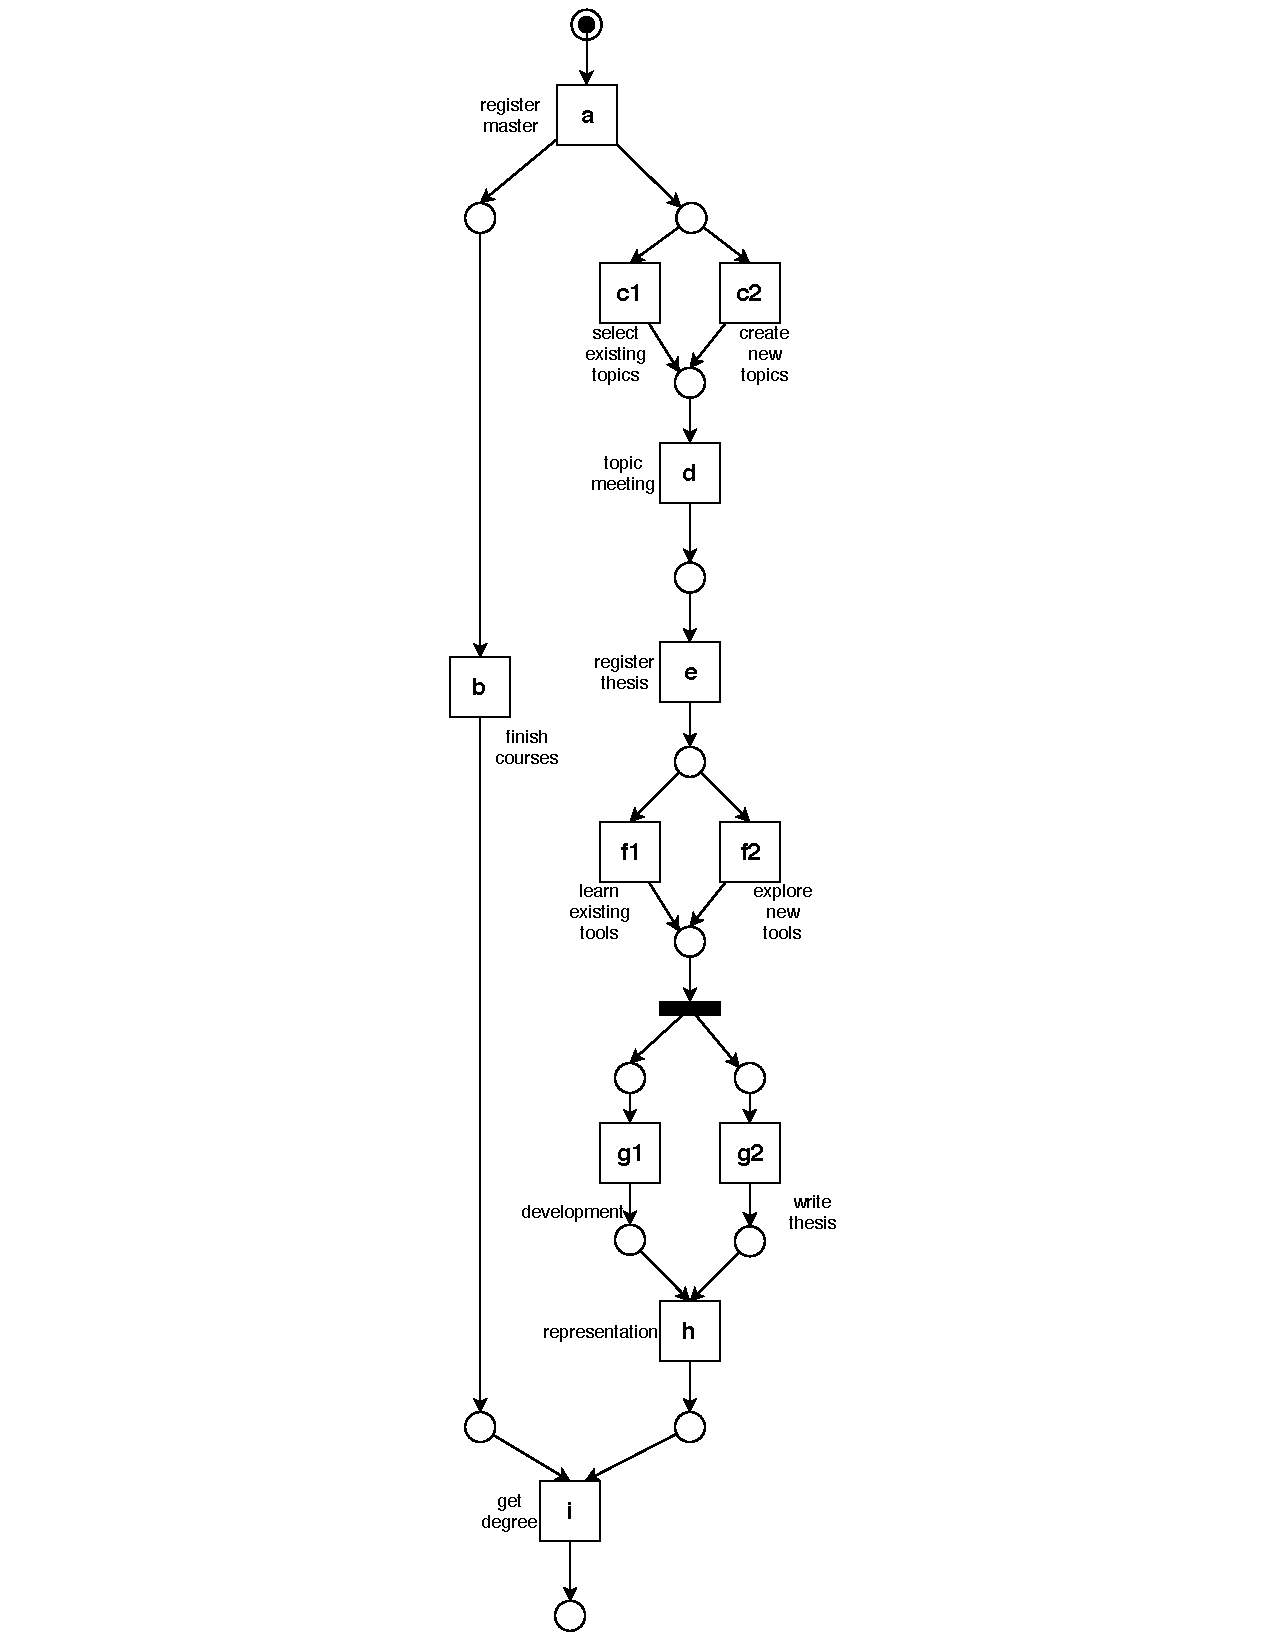
\includegraphics[clip, trim=7cm 0cm 7cm 0cm, width=0.4\textwidth, height=0.7\textheight]{figures/introduction/Master-original-model.pdf}
	\caption{original master study process $M_0$}
	\label{fig:model_M0}
\end{wrapfigure}
% In this section, we use thesis registration example to display the shortcomings of existing techniques and then introduces our methods, but we need to answer them later..
This section describes some situations where current repair techniques tend to fail. For the sake of understanding, examples are extracted from the common master study procedure to illustrate those situations.

The main activities for the master study include \emph{register master}, \emph{finish courses} and \emph{write a master thesis}. Here, we simplify the \emph{finish courses} and only extend the activity \emph{write a master thesis} into a set of sub activities. Those activities are shown in the Petri net model $M_0$ of Figure \ref{fig:model_M0}. The activities are modeled by the corresponding \textbf{\emph{transitions}} which is represented by a square. Transitions are connected through a circle called \textbf{\emph{place}}. Transitions and places build the static structure of Petri net and describe the transition relations. \textbf{\emph{Tokens}} in the black dot are put in the initial places and represent the dynamic state of the model. 

$M_0$ is currently in an initial state where only one token is at the start place to enable the transition \emph{register master}. After firing \emph{register master}, the token at the initial place is consumed while two new token are generated in the output places of \emph{register master}. In this way, activity \emph{finish courses}  can be executed concurrently the other branch except for the \emph{get degree}. When multiple activities have the same input place, all of them are enabled but only one of them can be fired and executed, namely, they are exclusive to each other. As shown in the figure,  \emph{select existing topics}  and \emph{create new topics} are exclusive, and only one of them can be triggered. When a transition has multiple input places, it can be triggered with condition that all input places hold at least a token. \emph{Get degree} is enabled only after \emph{finish courses} and \emph{representation} done. 


% here we are going to talk about the situations where the current repair method can not handle well.
%talk about the execution trace definition. 
% but how to combine them into one example?? I don't think it clearly here. But I need to show it later.
Along the tokens flowing through the model, activities get fired and generate a sequence according to their execution order. One execution sequence is called a trace. A set of traces depicts the model behavior and is recorded into a data file called event log. In real life, activities might be executed with deviation to the process model. A trace which has no deviation to the model is fitting. Otherwise, it's a unfitting trace. With accumulation of deviations, process model needs amending to reflect reality.  In the following part, different several situations are introduced to demonstrate the shortcomings of current techniques to repair a model. 
\subsection{Situation 1: \small{Repairing Model with Unfitting Traces}} % add preparation to this model
In some universities, before registering a master thesis, the activities \emph{write proposal} and \emph{check course requirement} with exclusive choice relation might be necessary in the master study procedure. The real process are recorded in the event log $L_1$. Traces with either of those activities are considered as positive. For convenience, alphabet characters are used to represent the corresponding activities and annotated in the model. \textbf{x1, x2} represent the activities \emph{write proposal} and \emph{check course requirement}.
\emph{Event Log $L_1$ -- }
		\begin{align*}
		Positive:\{ & { <a,b, c1,d,e,\textbf{x1},f1,g1,g2,h,i>}^{50}, \\   &{<a,b, c2,d,e,\textbf{x2},f2,g2,g1,h,i>}^{50} \}
		% Negative: \{ & {<a,c1,d,\quad f,g1,g2,h,i>}^{50} \}
		\end{align*}
\begin{figure}[htp]
	\centering
	\begin{subfigure}[b]{0.5\textwidth}
		\centering
		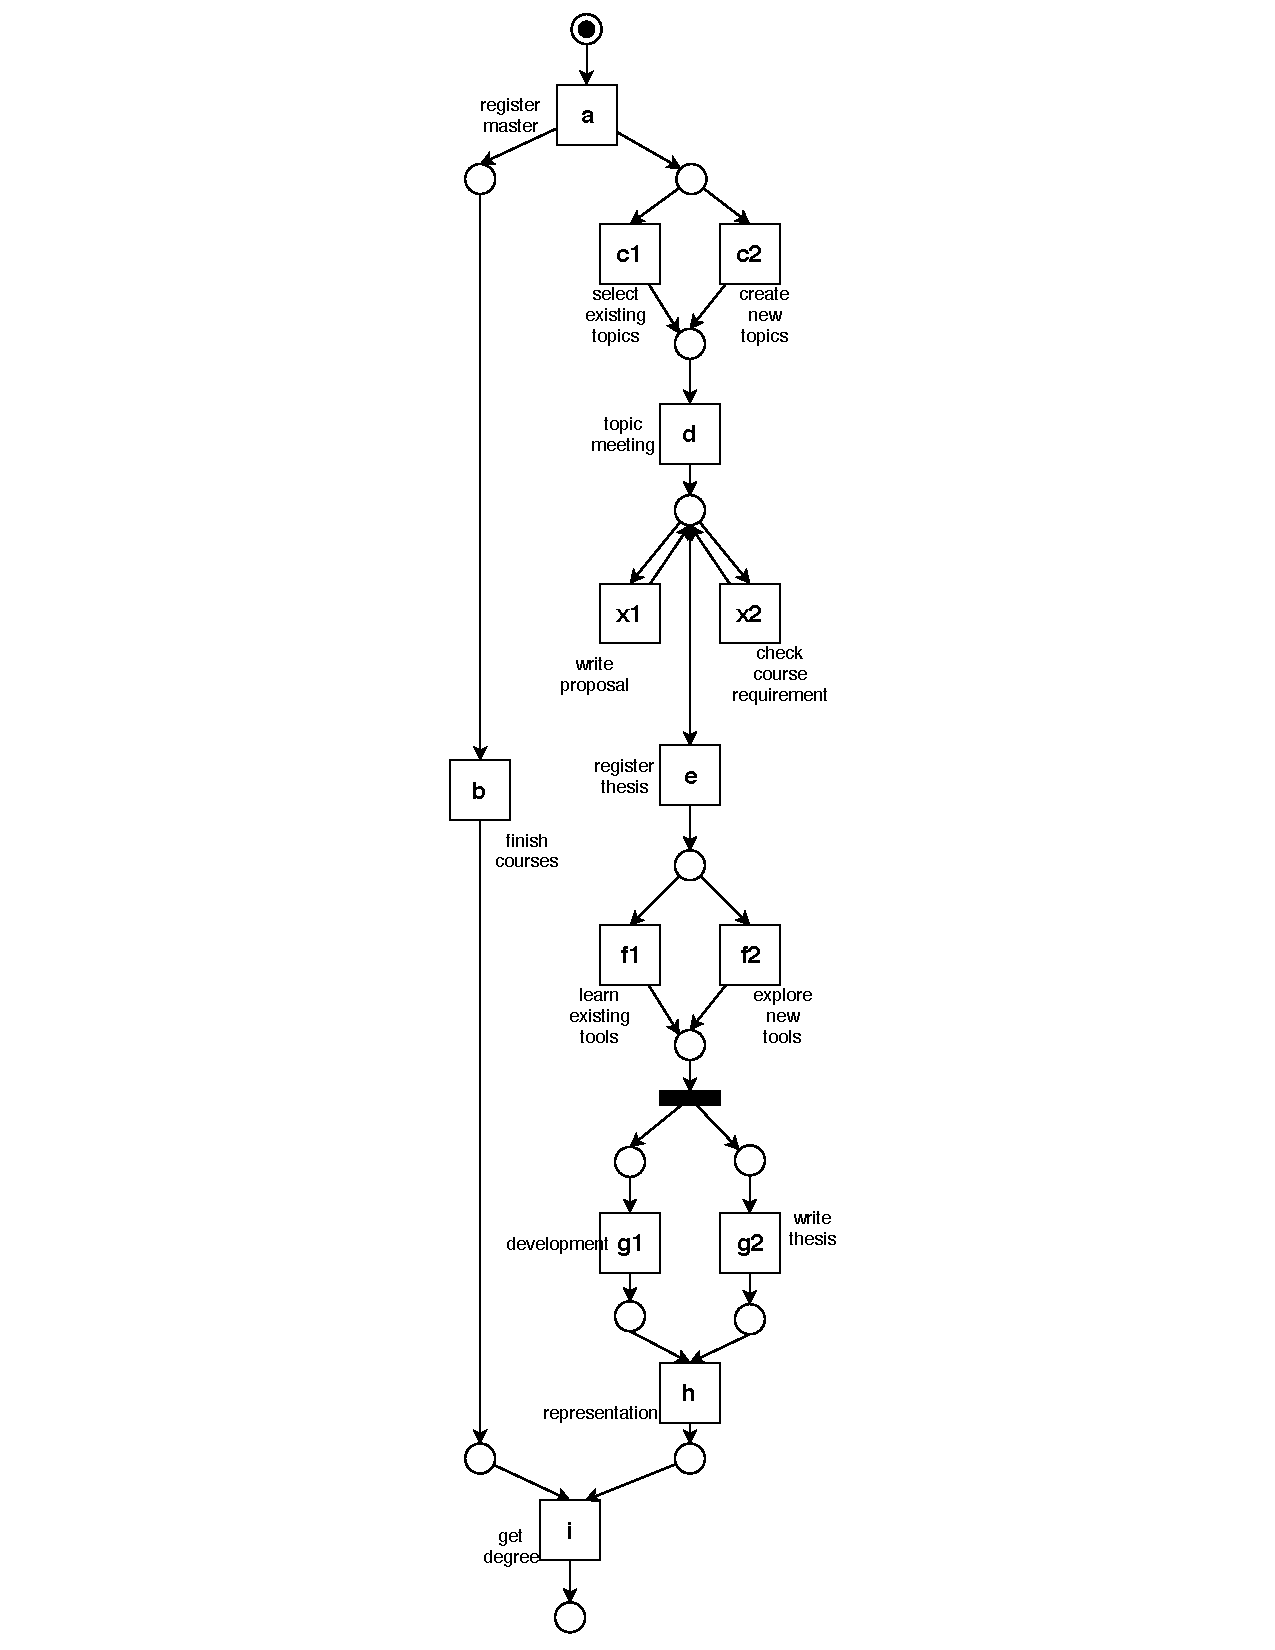
\includegraphics[clip, trim=7cm 0cm 7cm 0cm, width=0.5\linewidth, height=0.7\textheight]{figures/introduction/Master-add-events-loop.pdf}
		\caption{repaired model $M_{1.1}$ with additional activities }
		\label{fig:model_b1}
	\end{subfigure}%
	\begin{subfigure}[b]{0.5\textwidth}
		\centering
		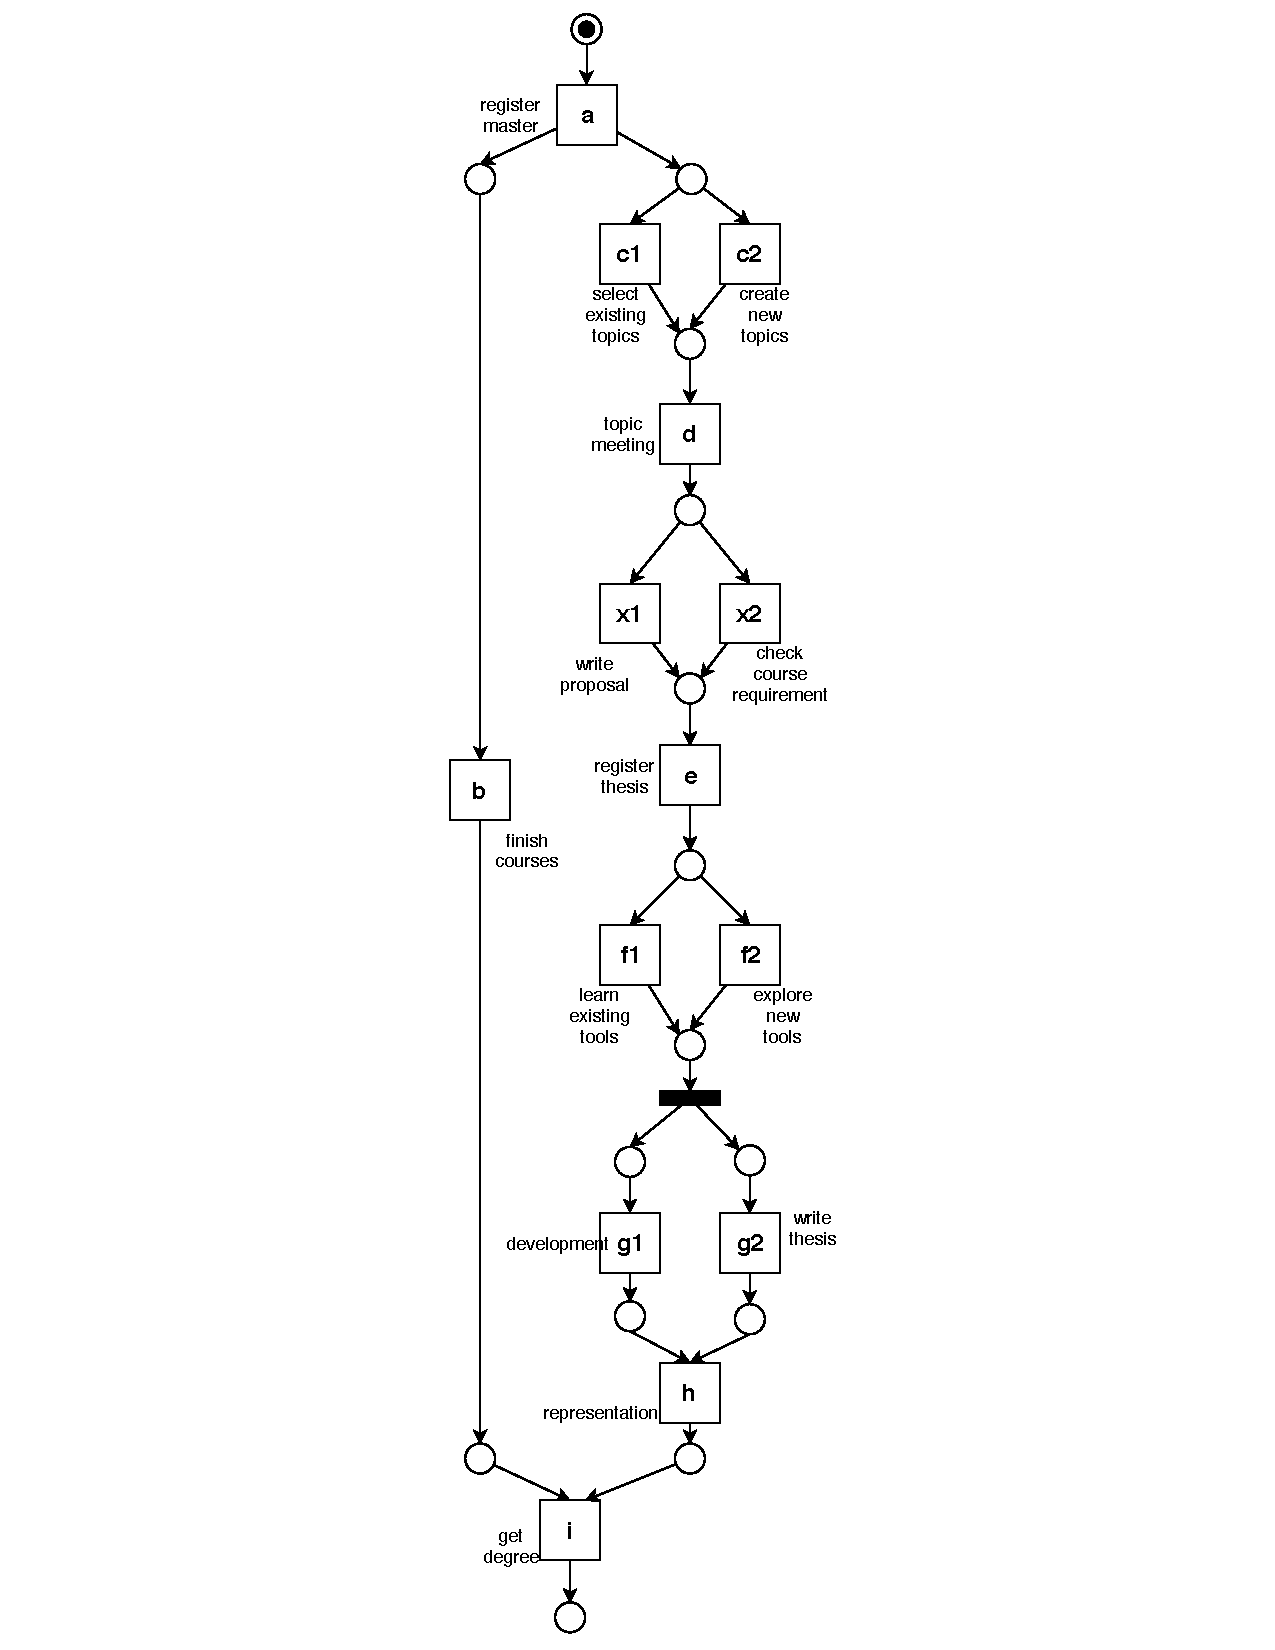
\includegraphics[clip, trim=7cm 0cm 7cm 0cm, width=0.5\linewidth, height=0.7\textheight]{figures/introduction/Master-add-events.pdf}
		\caption{expected model $M_{1.2}$ with additional activities}
		\label{fig:model_b2}
	\end{subfigure}
	\caption{example for situation 1 where $M_{1.1}$ is repaired by adding subprocess in the form of loops, which results in lower precision compared with the expected model $M_{1.2}$.}
	\label{fig:model_change_1}
\end{figure}

Because the existing repair techniques \cite{fahland2015model} don't consider the performance of traces in event log, all instances with positive labels are used to repair the model. Firstly, the deviations of the existing model M0 and the event log $L_1$ are computed. After computation of deviations, each deviation has the same start and end place and two deviations appear at the same position in the model. When repairing this model, each subprocess has one place as its start and end place, which forms a loop in the model. If there is only one such subprocess, the subprocess is added in a sequence in the model, which leads to a higher precision. Yet the algorithm does not discover orderings between different subprocesses at overlapping locations. So the subprocesses are kept in a loop form. 

The repaired model is shown in Figure \ref{fig:model_b1}, where the two additional activities are added in the form of loop. The repair algorithm in \cite{dees2017enhancing} builds upon \cite{fahland2015model} and considers the performance of the event log. However, the repaired model is the same as the one in Figure \ref{fig:model_b1}. The reasons are: (1) there is no deviation from negative factors. (2) positive deviations are used in the same way as \cite{fahland2015model}. 

Compared to the model in Figure \ref{fig:model_b1} where the two extra activities are shown in loop, the model in Figure \ref{fig:model_b2} are more expected, since it includes the two activities in sequence and has a higher precision.

\subsection{Situation 2: \small{Repairing A Model with Fitting Traces}}
% we should delete the prepare carefully and casually from the model. Only consider to add the data about the order change..what we expect is not 
This situation describes the existing problem in the current methods that fitting traces with negative performance outcomes cannot be used to repair a model. Given an actual event log $L_2$, when activity \emph{finish courses} is fired after \emph{begin thesis} and before writing master thesis, it reduces the pressure for the master thesis phase and traces in such an order are treated as positive. Else, the negative outcomes are given. 
\emph{Event Log $L_2$ -- }
\begin{align*}
Positive:\{ & { <a,\textbf{b},c1,d,f,g2,g1,h,i>}^{50}, \\   &{<a,\textbf{b},c2,d,f,g1,g2,h>}^{50} \}  \\
Negative: \{ & {<a,c1,d,f,g2,g1,\textbf{b},h,i>}^{50}, \\
& {<a,c1,\textbf{b},d,f,g1,g2,h,i>}^{50},  \}
\end{align*}
Compared to the model, the event log $L_2$ contains no deviations. When we apply the techniques in \cite{fahland2015model} and \cite{dees2017enhancing} to repair the model, the model keeps untouched due to no deviation. Apparently, the reason that those two methods can't incorporate the negative information in fit traces causes this shortcoming. When we expect a model which enforce the positive instances and avoid the negative instance as the model $M_2$, the current methods don't allow us to obtain such results. 
\begin{figure}[htp]
	\centering
	\begin{subfigure}[b]{0.5\textwidth}
		\centering
		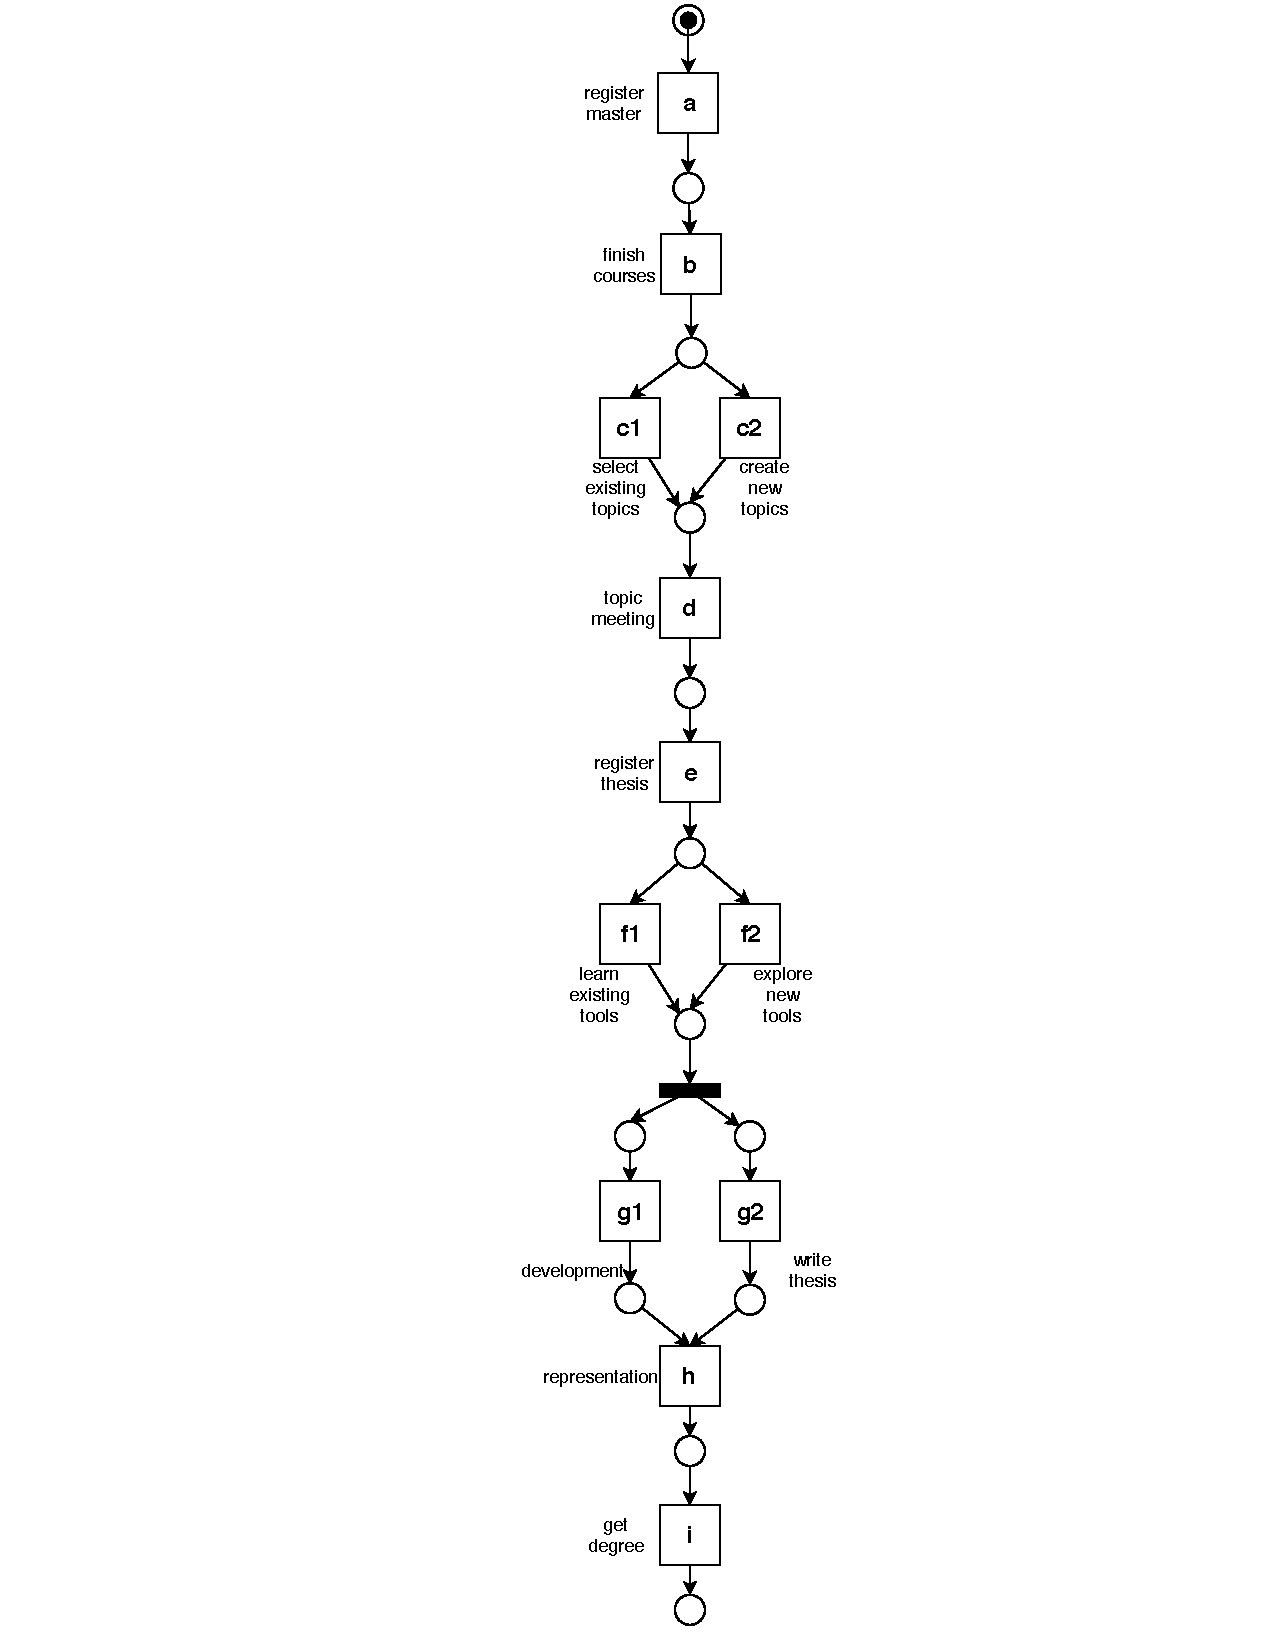
\includegraphics[clip, trim=8cm 0cm 8cm 0cm, width=0.5\linewidth, height=0.7\textheight]{figures/introduction/Master-change-order.pdf}
		\caption{expected model $M_{2}$ with order change}
		\label{fig:model_c}
	\end{subfigure}%
	\begin{subfigure}[b]{0.5\textwidth}
		\centering
		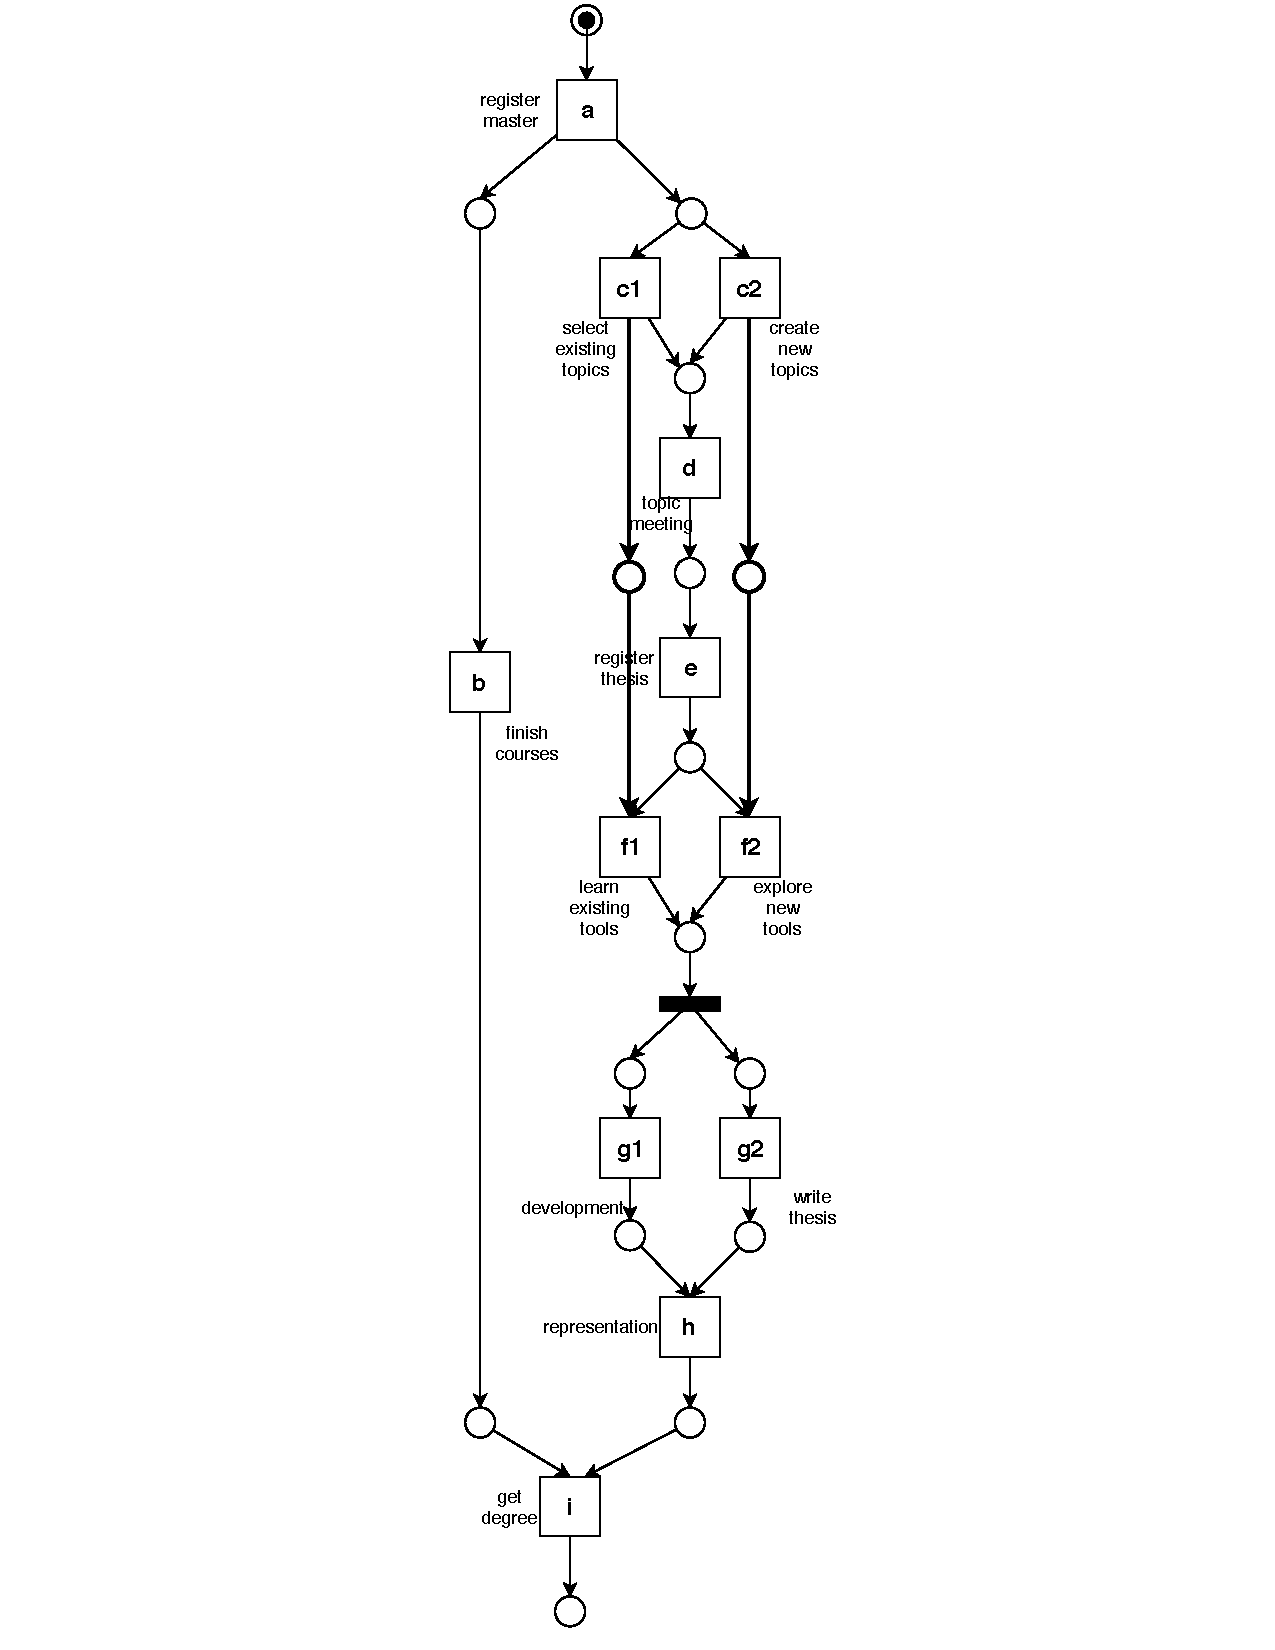
\includegraphics[clip, trim=7cm 0cm 7cm 0cm, width=0.5\linewidth, height=0.7\textheight]{figures/introduction/Master-with-lt.pdf}
		\caption{model $M_{3}$ with long-term dependency}
		\label{fig:model_d}
	\end{subfigure}
	\caption{example for situation 2 and 3}
	\label{fig:model_changes_2_3}
\end{figure}
\subsection{Situation 3: \small{detect long-term dependency}}
This part introduces a problem which causes a lower precision in process mining. It is the inability in current methods to detect the long-term dependency in the Petri net. The long-term dependency describes the phenomenon that one execution choice decides the execution of activities that do not follow directly. Due to the long distance of this dependency, current methods cannot detect it and improve the precision by adding long-term dependency on the model. 
An event log $L_3$ is given in the following. By using time consumption as one KPI, if the total sum goes over one threshold, we mark this trace as negative, else as positive. Since the activity \emph{create new topics} usually demands new knowledge rather than checking the existing tools. So if students choose to learn existing tools, it's possibly not useful and time is wasted. In the other case, if we select existing topics with existing background, it saves time when we directly learn the existing tools. According to this performance standard, we classified those event traces.
\emph{Event Log $L_3$ -- }
\begin{align*}
Positive:\{ & { <a,b,\textbf{c1},d,e,\textbf{f1},g1,g2, h,i>}^{50}, \\   &{<a,b,\textbf{c2},d,e,\textbf{f2},g2,g1, h,i>}^{50} \}  \\
Negative: \{ & {<a,b,\textbf{c1},d,e,\textbf{f2},g2,g1,h,i>}^{50}, \\
& {<a,b,\textbf{c2},d,e,\textbf{f1},g1,g2,h,i>}^{50}  \}
\end{align*}
%here we list one example to explain the long-term dependency, but we need to make them clear, might without the loop item..It means that we need to change the whole model..
There are no deviations of the model and event log $L_3$ according to the  algorithms in \cite{fahland2015model} and \cite{dees2017enhancing}. Therefore, the original model stays the same and allows for the execution of negative instances. After checking the model and log, those long-term dependencies have significant evidence. Transition \textbf{\emph{c1}} decides \textbf{\emph{f1}} while \textbf{\emph{c2}} decides \textbf{\emph{f2}}.  After addressing long-term dependency like the model $M_3$ in Figure \ref{fig:model_d} by connecting transitions to extra places, 
negative instances are blocked and the model has higher precision.

Clearly, the use of negative information can bring significant benefits, e.g, enable a controlled generalization of a process model: the patterns to generalize should never include negative instances. The demand to improve current repair model techniques with incorporating negative instances appears. In the next section, the demand is analyzed and defined in a formal way.

\section{Research Scope And Questions }
After analyzing the current model repair methods, we limit our research scope as shown in Figure \ref{fig:scope}.  The inputs for our research are one existing process model M, an event log L . According to predefined KPIs, each trace in event log is classified into positive or negative. After applying repair techniques in the black box, the model should be improved to enforce the positive instances while disallowing negative instance, with condition that the generated model should be as similar to the original model as possible. 
\begin{figure}
	\centering
	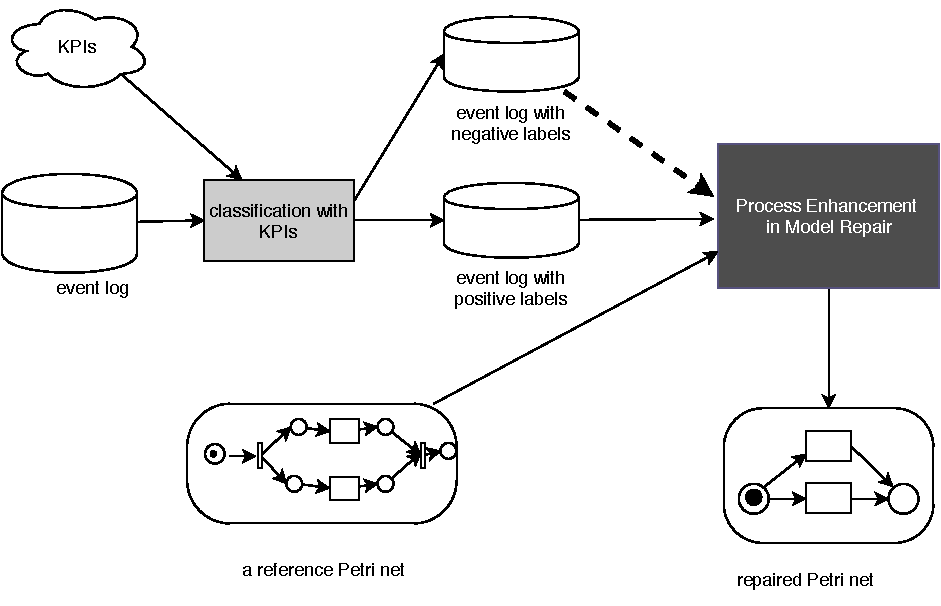
\includegraphics[width=\textwidth]{figures/introduction/P06-problem-scope.pdf}
	\caption{The problem description}
	\label{fig:scope}
\end{figure}

In this scope, we come up with several research questions listed in the following.
\begin{enumerate}[start=1,label={\bfseries{ RQ\arabic*:}}]
	%\itemsep0em
	\item How to overcome the shortcomings of current repair techniques in situations 1-3 above?
	\item How to balance the impact of the existing model, negative and positive instances together to repair model? 
	\item How to block negative instances from the model while enforcing the positive ones?
\end{enumerate}
  
In the remainder, we propose a solution for the black box. It analyzes process performance on trace level and balances the existing model, positive traces and negative traces on directly-follows relation, in order to incorporate all the factors on model generation. 

\section{Outline}
This thesis tries to answer the questions presented in section 1.2 in the remainder chapters and provide a solution for the black box. 
Chapter 2 and 3 introduces the related work and recalls the basic notions on process mining and list the preliminary to solve the problem. 
Chapter 4 describes the algorithm to solve the problem. 
In Implementation part, screenshots are given from the finished tools of our algorithm to demonstrate the use.  Experiment chapter answers the last question RQ3, by conducting a bundle of experiments. Later, results are analyzed and discussed. 
The last chapter is the summary of our work. 
%The next section answers the questions, how to balance all factors and block negative instances, Our algorithm analyzes process performance on trace level and balances the existing model, positive traces and negative traces on directly-follows relation, in order to incorporate all the factors on model generation. Long-term dependency is further detected on the intermediate model and added to block negative instances. What's more, the impact of the existing model, positive and negative instances are parameterized by weights, to allow more flexibility of the generated model.



%\end{document}

\iffalse
\chapter{Related Work} \label{chap:backgrd}
%% we should write the inductive miner , directly-follows relation in this paper,
%% but how to organize them together??
To update an existing process model in organizations, there are two strategies, rediscovery and process enhancement. Process rediscovery applies the discovery techniques on the actual event log to mine a new model. Process enhancement improves the model based on not only the actual event log but also the existing model. 


Process discovery has been intensively researched in the past two decades and many algorithms have been proposed \cite{van2016data}. Directly-follows methods \cite{van2004workflow, leemans2013discovering} investigate the  order of activities in the traces and extract higher relations which are used subsequently to build process models. State-based methods like  \cite{bergenthum2007process, cortadella1995synthesizing}  build a transition system to describe the event log, and then group the state regions into corresponding Petri net node. Language-based algorithms uses integer linear system to represent the place constraint where the token at one place can never go negative. By solving the system, a petri net is created. Its representative techniques are Integer Linear Programming(ILP) Miner \cite{van2008process}. Other methods due to  \cite{van2009process} include search-based algorithms, like Genetic Algorithm Miner \cite{de2007genetic}, and heuristic-based algorithms, like Heuristics Miner \cite{weijters2003rediscovering}. 

Among those discovery methods, Inductive Miner is widely applied \cite{leemans2013discovering}. It investigates the activity order in the traces and represents the order in a directly-follows graph. Based on the graph, it finds the most prominent split from the set of exclusive choice, sequence, parallelism, and loop splits on the event log.  Afterward, the corresponding operator to the split is used to build a block-structured process model called a process tree. Iteratively, the  split sublogs are passed as inputs for the same procedure until one single activity is reached and no split is available. The mined process model is a process tree that can be converted into the classical process model Petri net. 


When the actual event log differs a lot from the referred process model, it is suitable to use the rediscovery method to improve the business execution. However, in some cases, the process enhancement focuses to extend or improve an existing process model by using an actual event log \cite{van2011process}. Besides extending the model with more data perspectives, model repair is another type of enhancement. It modifies the model to reflect observed behavior while keeping the model as similar as possible to the original one.

In  \cite{fahland2012repairing}, model repair is firstly introduced into process enhancement. By using conformance checking, the deviations of the event log and process model are detected. The consecutive deviations in log  are only collected in the form of subtraces at a specific location Q in the model. Later, the subtraces are grouped into sublog that share the same location Q for subprocess discovery. In the earlier version in  \cite{fahland2012repairing}, the sublogs are obtained in a greedy way, while in  \cite{fahland2015model}, sublogs are gathered by using ILP Miner to guarantee the fitness. Additional subprocesses are introduced into the existing model to ensure that all traces fit the model, but it introduces more behavior into the model and lowers the precision.

Later, compared to  \cite{fahland2012repairing, fahland2015model}, where all deviations are incorporated in model repair,  \cite{dees2017enhancing} considers the impact of negative information.  In  \cite{dees2017enhancing}, the deviations of the model and event log are firstly analyzed, in order to find out which deviations enforces the positive performance. Given a trace and a selected KPI, an observation instance is built to correlate  activities in event logs which are deviating from models. Based on the observation instance,  a set of rules are derived in the form of a decision tree. According to the rules, the original event log is divided into sublogs with traces matching the rules. The sublogs are then repaired with trace deviations which lead to positive KPI outputs. Following repair, the sublogs are merged as the input for model repair in  \cite{fahland2015model}. According to the study case in  \cite{dees2017enhancing}, \cite{dees2017enhancing} provides a better result than  \cite{fahland2015model} on the aspect of performance. 
 
As described above, the state-of-the-art repair techniques are based on positive instances, meanwhile, the negative information is neglected. Without negative information, it is difficult to balance the fitness and precision of those model. Likewise, little research gives a try to incorporate negative information in multiple forms on process discovery.

In  \cite{goedertier2009robust}, the negative information is artificially generated by analyzing the available event set before and after one position and represented in the form of the complement of positive event sets. Based on the positive and negative event sets, Inductive Logic Programming is applied to detect the preconditions for each activity. Those preconditions are then converted to Petri net after applying a pruning and post-process step. Similar work on model discovery based on artificial negative events are published later. In  \cite{vanden2014determining}, the author improves the method in  \cite{goedertier2009robust} by assigning weights on artificial events with respect to an unmatching window, in order to offer generalization on the model. 

The work in  \cite{ponce2016incorporating} uses traces in the event log with negative outcomes as negative information. It extends the techniques of numerical abstract domains and Satisfiability Modulo Theories(SMT) proposed in  \cite{carmona2014process} to incorporate negative information for model discovery. Each trace  as positive or negative is transformed as one point in n-dimensional space, n is the number of distinct activities. By adding places between transitions, it limits the transition execution by demanding tokens on those added places. This limit can be reflected by the sequence of traces.  In linear system, those limits are represented into a set of inequalities and in a form of convex polyhedron in n-dimensional space. Given half-space hypotheses, SMT solves the inequalities and gives the limits on the process model. Before SMT, negative information is incorporated to shift and rotate the polyhedron, which limits the generalization of the solution space. Because half-space is used, this method can not deal with negative instances overlapped on positive instances.


However, the field of model repair which considers the negative information is new. Furthermore, the idea to incorporate negative instances on trace level into model repair is innovative.  

\iffalse
Compared to this, our approach is innovative mainly in the following aspects. 
\begin{itemize}
	\item Incorporate the negative information into model repair. 
	\item Analyze the long-term dependency in the model to provide a preciser result. 
	\item Analyze Model on Trace level. All activities constituting a trace are considered. 
\end{itemize}
\fi



\chapter{Preliminaries} \label{chap:prelim}\pagenumbering{arabic}
% we should list the event log definition and petri net definition
% also the process tree definition
This chapter introduces the most important ground concepts and notations that are used in the remainder of this article. Firstly, the data and process models in process mining are described; Later, one related discovery technique is introduced.
\section{Event Log}
% introduce of event and trace , later event log historical business process execution data in information systems
Business process in organizations is reflected by its execution of a set of activities. The historical execution data is usually in a form of event logs in information systems and can be used by Process Mining to analyze the business execution. To specify the event log, we begin with formalizing the various notations\cite{van2016data} .
\begin{definition}[Event]
	An event corresponds to an activity in business execution and can be marked by $e$. An event is characterized by attributes, like a timestamp, name, and associated costs, etc. The finite set of events in the process is written as $\mathcal{E}$.
\end{definition}
\begin{definition}[Trace]
A trace is a finite sequence of events $\sigma \in \mathcal{E}^*$ with conditions that \emph{(i)} each event can not appear twice in a trace, $ \forall i,j, 1 \leq i,j \leq \vert \sigma \vert, if \ i \neq j, then\ \sigma (i) \neq \sigma (j) $.  \emph{(ii)} one event can only appear in one trace, $ \forall e \in \sigma, if\ e \in \sigma\prime, then\ \sigma = \sigma\prime $. 
A trace also has a set of attributes, which describes the trace characters, like the identifier, the trace cost.
\end{definition}
\begin{definition}[Event Log]
An event log $L$ is a set of traces. If an event log contains timestamps, then the ordering in a trace should respect these timestamps. 
\end{definition}
\section{Process Models}
After gathering the event log from information systems, process mining can discover a process model based on the event log, aims to improve understanding and insights on the business process. Multiple process modeling languages are applied in process mining in the last years, such as Petri net, BPMN models, etc. Petri nets are bipartite graph to describe concurrent systems. BPMN models, fully named Business Process Model and Notation models, include many different elements and are flexible but complex tool to visualize business process. Process tree is based on a tree structure to organize the event relation. In this article, due to simplicity, we focus on Petri net and process tree.
\subsection{Petri Net}
Among multiple models which are proposed to describe the process, Petri net has been best studied to allow for the modeling of concurrency. 
\begin{definition}[Petri net]
	A Petri net N is composed of a finite set of places P, transitions T, and a set of directed arcs $F \subseteq (P \times T) \cup (T \times P)$, which can be written as $N=(P,T,F)$. A marked Petri net is (P,T,F,M) where M the marking of the net. A marking of a net N is a multi-set over P, $M \in \mathbb{P} $. 
\end{definition}
An example is shown in Figure \ref{fig:pn-seq-2}. It has transitions $T=\{A,B,C,D,E\}$ and four places with the initial marking in the place before $T=\{A,B\}$. 
\begin{figure}[!h]
	\centering
	\begin{subfigure}[b]{0.45\textwidth}
		\centering
		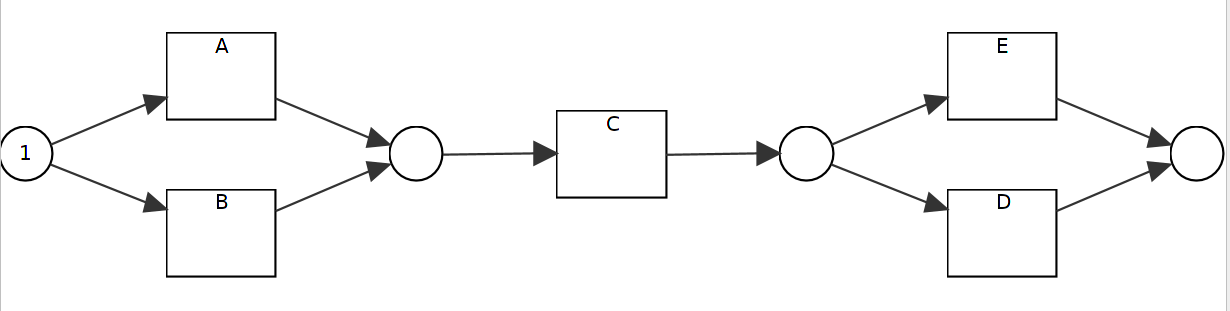
\includegraphics[width=\linewidth]{figures/preliminary/PN06_Seq_2_xor_notnested.png}
		\caption{A Simple Petri net}
		\label{fig:pn-seq-2}
	\end{subfigure}%
	\quad
	\begin{subfigure}[b]{0.45\textwidth}
		\centering
		\includegraphics[width=\linewidth]{figures/preliminary/PT06_Seq_2_xor_notnested.png}
		\caption{A process tree corresponding to Fig \ref{fig:pn-seq-2}}
		\label{fig:pt-seq-2}
	\end{subfigure}%
\end{figure}
%% Here add the definition for silent transitions 
\subsection{Process Tree}
Process tree is block-structured and sound by construction, while Petri nets, BPMN models possibly suffer from deadlocks, other anomalies\cite{van2016data}. Here we give the definition of process tree.
\begin{definition}[Process Tree]
Let $ A \subseteq \mathbb{A} $ be a finite set of activities with silent transition $\tau \in \mathbb{A}$, $\bigoplus \subseteq \{\rightarrow, \times, \land, \circlearrowright\}$ be the set of process tree operators. 
\begin{itemize}
\item $Q=a$ is a process tree with $a\in A$, and 
\item $Q= \oplus (Q_1 , Q_2 ,.. Q_n)$ is a process tree with $\oplus \in \bigoplus$, and $Q_i$ is a process tree, $i\in{1,2,..,n}, n\in \mathbb{N}$. 
\end{itemize}
\end{definition}

Process tree operators represents different block relation of each subtree. Their semantics are standardized from \cite{vanderAalst:2016:PMD:2948762, Buijs2012OnTR} and explained with use of Petri net in Figure \ref{fig:pn_pt_correspondings}\cite{Buijs2012OnTR}.
\begin{figure}[!h]
	\centering
	\begin{subfigure}[b]{0.45\textwidth}
		\centering
		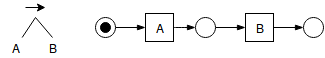
\includegraphics[width=\linewidth]{figures/preliminary/PT_PN_corresponding_01_seq_PN.png}
		\caption{Sequence}
		\label{fig:pt_pn_seq}
	\end{subfigure}%
	\quad
	\begin{subfigure}[b]{0.45\textwidth}
		\centering
		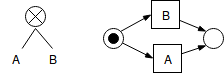
\includegraphics[width=\linewidth]{figures/preliminary/PT_PN_corresponding_02_xor_PN.png}
		\caption{Exclusive choice}
		\label{fig:pt_pn_xor}
	\end{subfigure}%
	\\ %this makes much difference
	\begin{subfigure}[b]{0.45\textwidth}
		\centering
		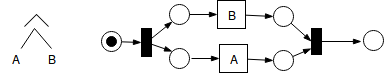
\includegraphics[width=\linewidth]{figures/preliminary/PT_PN_corresponding_03_and_PN.png}
		\caption{ Parallelism }
		\label{fig:pt_pn_and}
	\end{subfigure}%
	\quad
	\begin{subfigure}[b]{0.45\textwidth}
		\centering
		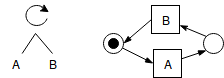
\includegraphics[width=\linewidth]{figures/preliminary/PT_PN_corresponding_04_loop_PN.png}
		\caption{Loop}
		\label{fig:pt_pn_loop}
	\end{subfigure}%
	\caption{Semantics of process tree operators w.r.t. Petri net}
	\label{fig:pn_pt_correspondings}
\end{figure}
\begin{definition}[Operator Semantics] 
	The semantics of operators $\bigoplus \subseteq \{\rightarrow, \times, \land, \circlearrowright \}$ are,
	\begin{itemize}
		\item if $Q= \rightarrow(Q_1 , Q_2 ,.. Q_n)$, the subtrees have sequential relation and are executed in order of $Q_1,Q_2,..Q_n$
		\item if $Q= \times(Q_1 , Q_2 ,.. Q_n)$,  the subtrees have exclusive choice relation and only one subtree of $Q_1,Q_2,..Q_n$   can be executed.
		\item if $Q= \land (Q_1 , Q_2 ,.. Q_n)$,  the subtrees have parallel relation and $Q_1,Q_2,..Q_n$ they can be executed in parallel.
		\item if $Q= \circlearrowright(Q_1 , Q_2 ,.. Q_n)$,  the subtrees have loop relation and $Q_1,Q_2,..Q_n \; with\; n\geq2$, $Q_1$ is the do-part and is executed at least once, $Q_2,..Q_n$ are redo part and have exclusive relation.
	\end{itemize}
\end{definition}
According to the corresponding semantic relations,  a process tree can be easily transformed into Petri net. In Figure \ref{fig:pt-seq-2}, it is the process model in process tree which describes the same process as in Figure \ref{fig:pn-seq-2}. 
%% here to describe the inductive miner 
\section{Inductive Miner}
To discover a process model from an event log, we choose one of the leading process discovery approaches -- Inductive Miner, because it guarantees the construction of sound model, and is flexible and scalable to event log data. Its steps are listed bellow. 
\subsection{Construct a directly-follows graph}
A the start, the event log $L$ is scanned to extract the directly follows relation of events. The directly-follows relation is like the one in $\alpha$-algorithm \cite{van2004workflow, leemans2013discovering}, but the frequency information is stored for each relation. Later, those relations are combined together to build a directly-follows graph with frequency. According to \cite{van2016data, leemans2013discovering}, a directly-follows graph is defined bellow.
\begin{definition}[Directly-follows Graph]
 The directly-follows relation $a > b$ is satisfied iff there is a trace $\sigma\ where, \sigma(i)=a \ and \ \sigma(i+1)=b$.
 A directly-follows graph of an event log $L$ is $G(L) = (A, F, A_{start}, A_{end}) $ where $A$ is the set of activities in L, $F={(a,b) \in A \times A | a >_L b} $ is the directly-follows relation, $A_{start}, A_{end}$ are the set of start and end activities respectively.
\end{definition}
The frequency information of the directly-follows relation is called cardinality and defined below.
\begin{definition}[Cardinality in directly-follows graph]
Given a directly-follows graph G(L) derived from an event log L, the cardinality of each directly-follows relation in G(L) is :  
	\begin{itemize}
		\item $Cardinality(E(A,B))$ is the frequency of traces with $\langle ...,A,B,... \rangle$. 
		\item Start node A cardinality $Cardinality(Start(A))$ is the frequency of traces with begin node A.
		\item End node B cardinality $Cardinality(End(A))$ is the frequency of traces with end node B.
	\end{itemize}	
\end{definition}
\subsection{Split Log Into Sublogs}
Based on the directly-follows graph, it finds the most prominent cut which is applied afterwards to split the event log into smaller sublogs. Cuts compose of \emph{exclusive-choice cut, sequence cut, parallel cut and redo-loop cut} which correspond to the process tree operators $ \{\rightarrow, \times, \land, \circlearrowright \}$. They are selected in the following order. A maximal exclusive-choice cut is firstly tried to split the directly-follows graph; if it is not available, then a maximal sequence cut, a  maximal parallel cut and a redo-loop cut are applied in sequence. Sublogs are created due to this available operator. Meanwhile, this operator is used to build the process tree. 

The same procedure is applied again on the sublogs until single activities. What's more, this process tree can be converted into Petri net for further analysis. 


\chapter{Algorithm} \label{chap:alg}
%% This is the main content about this article. I should list them in an order
%% How to balance the existing model, positive and negative instance together, I shall use the dfg-method to create a dfg-matrix to incorporate the impact.
%% how to introduce them into adding long-term dependency feature. After mining the model by Inductive Miner, we have a model without long-term dependency, but we need to change the model and give the right examples.. 
%% If we change the data set, then we need to change the model into another parts, but the current methods can not solve it..
%% Should we also separate them into different sections?? Yes, we need it
%% Also, to delete the silent transition, as one option feature in our methods, we only delete it, in this situation, which will not affect the model behavoirs.

%% Or we could organize the content in this way:
%%  -- put the whole structure ahead and put all that we want to talk
%%  -- list the steps 
%%    ++ dfg-method to balance the directly-follows relation and create the corresponding directly-follows graph
%%    ++ add long-term dependency on the model
%%    ++ delete the silent transitions on the model as a post model

%% Put some words here
This chapter begins with a general framework to repair a reference process model by incorporating the negative instances. A concrete algorithm within the framework is proposed in the subsequent sections. 
%our repair algorithm to incorporate the negative instances on process enhancement. In the beginning, the architecture of this algorithm is provided to give an overview. Details of main steps are represented in the following order. Firstly, the impact of the existing model, positive and negative instances are balanced in the media of the directly-follow relations. Inductive Miner is then applied to mine process models from those directly-follows relations. Next, we detect and add long-term dependency on the generated process models. Furthermore, the model in Petri net with long-term dependency is  post-processed for the sake of simplicity. 
\section{General Framework for Repairing Process Models}
%% Describe the 
Figure \ref{fig:framework} shows our proposed framework to repair a process model with negative information. The inputs are a reference process model and a labeled event log. The reference process model can be in multiple types, e.g. Petri net, process tree. Traces in the labeled event log are classified as positive or negative in respect to some KPIs of business processes. The output is a repaired process model with the same type as the reference model.

The basic idea behind the framework is to unify the impact from the reference model $M$, positive sublog $L^+$ and negative sublog $L^-$ into data models. Those data models are of the same type and denoted as $D^M$, $D^+$ and $D^-$ respectively. Then we consider all impact from models and generate a new data model $D^n$. $D^n$ is later transformed into a process model $M^r$ as the output. Several post-processes are optional to improve the repaired model $M^r$.

After defining a data model to unify the impact and implementing the process modules in the general framework, a solution which also considers the negative information on model repair is developed. 
\begin{figure}
	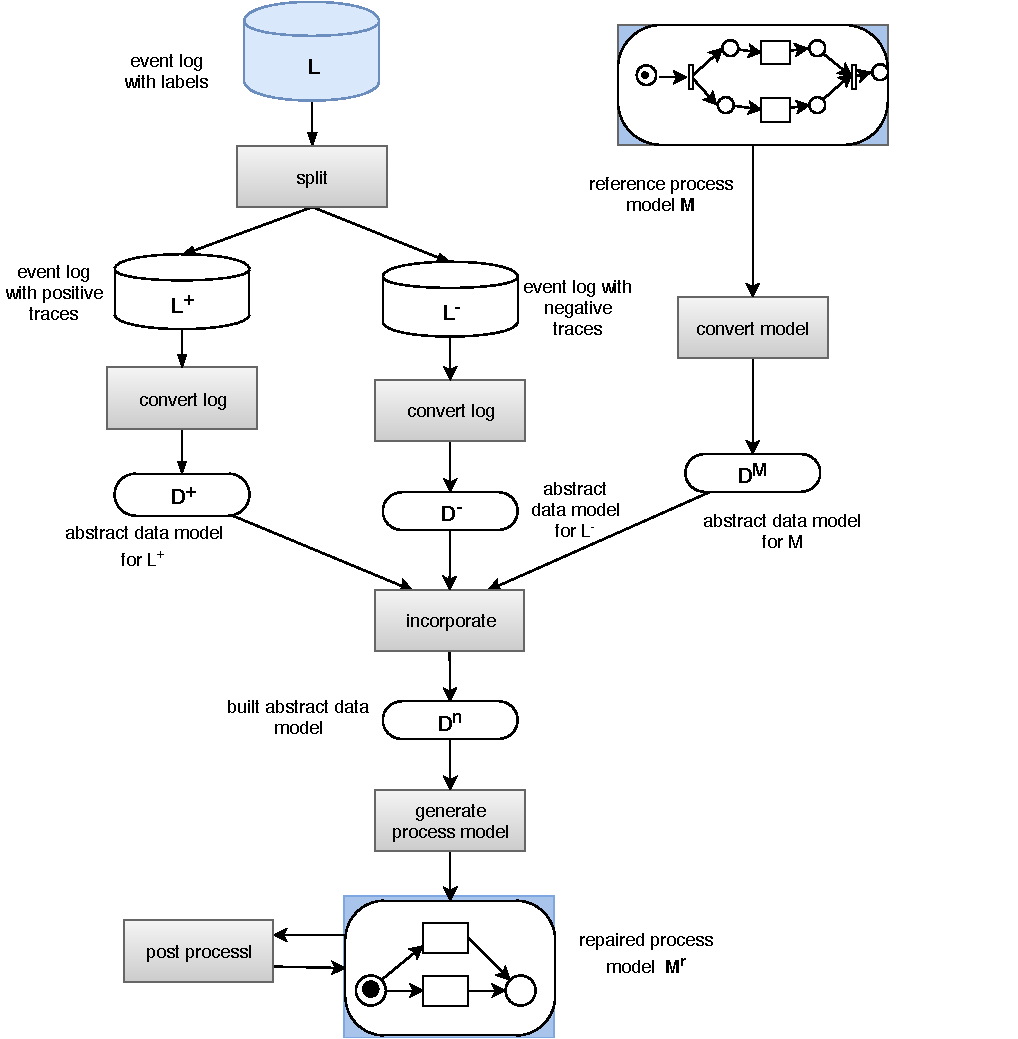
\includegraphics{figures/algorithm/FD_framework.pdf}
	\caption[Model Repair Architecture]{Model Repair Architecture -- \small Rectangles represents processes and data models in eclipse shape. Input event log and the reference model are in blue, while the repaired model is in green.}
	\label{fig:framework}
\end{figure} 
\section{Algorithm}
Given the inputs, an event log and a Petri net as the reference process model M, our task is to repair the referenced Petri net based on the actual event log with consideration of negative information. 

Based on those scope, the main modules in the framework in Figure \ref{fig:framework} is designed and developed to repair the reference Petri net. We denote our repair algorithm as \textbf{dfg-repair}. First of all, we define a proper data model to represent the impact from Petri net M, and the event log L. Then, we list all the modules  and describe our basic ideas to implement them. 
% here to point out our input and output
\subsection{Unified Data Model}
We choose the directly-follows graph as the basis of our unified data model to represent the impact from the reference model and the event log. The reasons are, (1) there exist transformation algorithms to extract a directly-follows graph from an event log and to convert directly-follows graph into process tree or Petri net, which saves our effort;(2) the cardinality of directly-follows graphs can be used to express the impact strength.

Although we can derive three directly-follows graphs from the reference model, the positive and negative event logs respectively, their cardinalities are in different level and not able to incorporate with each other. So we introduce a concept called unified cardinality to bring all the impact into the same level, which is the percentage to the sum of total cardinalities with a range [0-1].
% here we already changed the definitions for the unifications..now it became as the percentage of the cardinality to its whole cardinality. No matter negative or positive ones...we can do it, right? 
\begin{definition}[Unified cardinality] 
	\label{def:car-unification}
	Given a directly-follows graphs $G(L)  = (A, F , A_{start}, A_{end})$ for a model, the unification for this graph is a function  $u:F\rightarrow N $ that has the following definition: \\
	for each directly-follows relation $(a,b) \in F$,
	\[ u(a,b) = \frac{c(a,b)}{\sum_{(a^\prime,b^\prime) \in F} c(a^\prime,b^\prime)}\]
	for start activities $a \in A_{start}$, 
	\[ u(a) = \frac{c(a)}{\sum_{a^\prime \in A_{start}} c(a^\prime)} \]
	Similarly for end activities $a \in A_{end}$,
	\[ u(a) = \frac{c(a)}{\sum_{a^\prime \in A_{end}} c(a^\prime)} \]
\end{definition}
A directly-follows graph with unified cardinality is denoted as a unified directly-follow graph $D(L)=(A, F , A_{start}, A_{end}, u)$. After analyzing the positive , negative instances from event logs and the reference process model, $D(L_{pos})$, $D(L_{neg})$ and $D(L_{ext})$ are generated as the directly-follows graphs with unified cardinalities.
\subsection{Modules List}
After fixing the unified data models, in order to repair the reference model, the following list of modules are necessary. 
% should we add some steps here to say from which model to which model??
\begin{itemize}
	\item \emph{Split event log into positive and negative sublogs } \quad
	The event log $L$ is split into an event log $L^+$ with only positive traces and an event log $L^-$with negative traces.
	\item \emph{Convert event logs into unified directly-follows graphs, $D^+, D^-$}\quad 
	Two unified directly-follows graphs are generated respectively for the positive instance and negative instances from the event log.
	\item \emph{Convert reference model into unified directly-follows graph $D^M$}\quad 
	\item \emph{Incorporate unified directly-follows graphs} \quad
	Three unified directly-follows  graphs $D^M, D^+, D^-$ are combined into one single directly-follows graph $D^n$ after balancing their impact.
	\item \emph{Generate process models from $D^n$} \quad
	Process models are mined from the repaired data model $D^n$.
	\item \emph{Post process the repaired model} \quad
	Several post-processes are optionally applied on the generated process model, in order to improve the process model quality according to certain criteria.
	%Long-term dependency is detected on the intermediate models and finally added on the Petri net. To simplify the model, the reduction of silent transitions can be applied at the end.
\end{itemize}
In those modules,for the simplicity, we skip the details for the module \emph{Split event log into positive and negative sublogs}. The details of the concrete algorithms to implement other modules are provided in the subsequent sections.
\subsection{Convert Event Logs into Unified Directly-follows Graphs}
Given an event log, to retrieve its unified directly-follows graph, we need to obtain its directly-follows graph at first. There is an existing procedure \emph{IMLog2Dfg} from  \cite{leemans2013discovering}. \emph{IMLog2Dfg} traverses traces in the event log, extracts directly-follows relations of activities, and generates a directly-follows graph based on those relations. 

By applying \emph{IMLog2Dfg} separately on the event logs $L^+$ and $L^-$, we generate two directly-follows graphs $G(L_{pos})$ and $G(L_{neg})$.  In the next step, the cardinalities from those graphs are unified according to Definition \ref{def:car-unification} and become a part of unified data model $D(L_{pos})$ and $D(L_{neg})$

\subsection{Convert Reference Model into Unified Directly-follows Graph}
The basic idea behind this convert is to transform a reference process model into a directly-follows graph and then unify this directly-follows graph into $D^M$.


To generate a directly-follows graph from a Petri net, we investigate the execution order of activities with help of a transition system. % how ti helos
In a transition system, the set of activities directly before a state have to be executed to reach this state, while the activities after this state are enabled to execute only after reaching this state. This implies the set of the activities before the state is executed before the set after the state. By analyzing the transition system, directly-follows relations between activities are extracted and used later to a directly-follows graph for the reference model.

From the positive and negative event logs, we can get the cardinality for corresponding directly-follows graph to represent the strength of this directly-follows relation. However, when the existing model is transformed into  directly-follows graph $G(L_{ext})$, there is no point to assign cardinality on each edge. So we just set cardinality with 1 for each arc. Based on this cardinality assignment, we attain the unified data model $D^M$ for the reference Petri net.

\subsection{Incorporate Unified Directly-follows Graphs}
After the unification, the impact from the existing model, the impact from positive and negative instances are in the same level and represented in $D^M$,$D^+$, and $D^-$. 
The strategy to incorporate those three models is that directly-follow relations are added into the repaired data model $D^n$ if the total support from $D^M$ and $D^+$ exceeds the rejection force from $D^-$. The other directly-follows relations are rejected. Namely, we balance all impact by subtracting the unified cardinality of $D^-$ from the sum of unified cardinality in $D^M$ and$D^+$.
\begin{definition}[Incorporating method] For any directly-follows relation from $D^M$,$D^+$, and $D^-$, we balance all forces on it in the following way. 
	\begin{itemize}
		\item For one directly-follows relation, \[ u^{n}(a,b) =  u^{M}(a,b)+ u^{+}(a,b)  - u^{-}(a,b) \] 
		\item For a start activity $a \in A^{M}_{start} \cup A^{+}_{start} \cup A^{-}_{start}$,
		\[ u^{n}(a) =  u^{M}(a)+ u^{+}(a)  - u^{-}(a)\]
		\item For an end activity $a \in A^{M}_{end} \cup A^{+}_{end} \cup A^{-}_{end}$
		\[ u^{n}(a) =  u^{M}(a)+ u^{+}(a)  - u^{-}(a)  \]
	\end{itemize}	
%if $u^{n}(a,b) > 1 , u^{n}(a,b) =1$, if $u^{n}(a,b) < 0 , u^{n}(a,b) =0$; 
% $ u^{n}(a) > 1 \Rightarrow  u^{n}(a) =1 ; u^{n}(a) < 0 \Rightarrow  u^{n}(a) =0$;
\end{definition}
% here is only the incorporation method
%% Here we add the control weight on it
In the real life, there exists various needs to address the impact either from the existing model, the positive instances or the negative instances. To meet this requirement, three control parameters $w^{M}$,$w^{+}$, and $w^{-} \in [0,1]$ are assigned respectively to each unified cardinality from the existing model, and positive and negative instances. The weighted unification is modified in the way bellow. 
\begin{definition}[Weighted incorporating method]
Given the control weight $w^{M}$,$w^{+}$, and $w^{-} \in [0,1]$, the weighted incorporating method to balance forces from $D^M$,$D^+$, and $D^-$ for $D_{n}$ is defined below.
\begin{itemize}
	\item For one directly-follows relation, \[ u^{n}_{w}(a,b) =  w^{M} * u^{M}(a,b)+ w^{+} * u^{+}(a,b)  - w^{-} * u^{-}(a,b) \] 
	\item For a start activity $a \in A^{M}_{start} \cup A^{+}_{start} \cup A^{-}_{start}$,
	\[ u^{n}(a) =  w^{M} * u^{M}(a)+ w^{+} * u^{+}(a)  - w^{-} * u^{-}(a)\]
	\item For an end activity $a \in A^{M}_{end} \cup A^{+}_{end} \cup A^{-}_{end}$
	\[ u^{n}(a) =  w^{M} * u^{M}(a)+ w^{+} * u^{+}(a)  - w^{-} * u^{-}(a)  \]
\end{itemize}	
\end{definition}
By adjusting the weights of $w^{M}$,$w^{+}$, and $w^{-}$, different focus can be reflected by the model. For example, by setting $w^{M}=0, w^{+}=1,w^{-}=1$, the existing model is ignored in the repair, while  the original model is kept in situation $w^{M}=1, w^{+}=0,w^{-}=0$.

Next, we filter the directly-follows relation according to its weighted cardinality. If the cardinality over one certain threshold, it indicates a significant support to add this relation into the repaired data model $D^n$. By adding those directly-follows relation, we build a unified directly-follow graph $D^n$ over this threshold t. 
% here to explain the building method for the new data model and the way from it?? But should we do it here, or later?? 
%After getting the weighted unification, we can assign cardinality for the directly-follows graph $G_{new}$ by multiplying weighted unification with the total number of cardinalities of $G(L_{pos})$, $G(L_{neg})$ and $G(L_{ext})$. 
\subsection{Generate Process Models from $D^n$}
% generate dfg from unified one
% derive models from dfg
The result of the last step above is a unified directly-follows graph $D^n$ with weighted cardinality. To generate a process model from it, we convert $D^n$ firstly into a general directly-follows graph $G^n$. Analyzing the weighted cardinality, we transform the weighted cardinality by multiplying the number of traces in labeled event log.
%the sum of cardinalities of $G(L^{+})$, $G(L^-)$ and $G(L^{M})$.  


Later, based on $G^n$, an existing procedure called \emph{Dfg2ProcessTree} is applied to mine process models like process tree and Petri net \cite{leemans2013discovering}. It finds the most prominent split from the set of exclusive choice, sequence, parallelism, and loop splits on  a directly-follows graph.  Afterward, the corresponding operator to the split is used to build a block-structured process model called a process tree. Iteratively, the split sub graphs are passed as inputs for the same procedure until one single activity is reached and no split is available. A process tree is output as the mined process model and can be converted into another process model called Petri net.
%% To write the procedure for it 
\subsection{Post Procedure on the Process Model}
Due to the intrinsic characters of Inductive Miner, the dependency from activities which are not directly-followed can't be discovered. To improve precision of the generated model, we propose one post procedure to add the long-term dependencies to the model. Additionally, another post procedure to simplify the model is introduced by deleting redundant silent transitions and places.
\subsubsection{Add Long-term Dependency}
Obviously, long-term dependency relates to the structure of choices in process model, such as exclusive choice, loop and or structure. Due to the complexity of handling long-term dependency on or and loop structure, we skip them but focus only on the long-term dependency in \textbf{exclusive choice structure}. 

The generated process tree mined by Inductive Miner is used as an intermediate process model to detect long-term dependency.  A process tree is  (1) easy to extract the exclusive choice structure, since it is block-structured. (2) easy to transform a process tree to a Petri net as the final model.
%% Here we need to add the relation of process to the long-term dependency

An exclusive choice structure is represented as \textbf{\emph{xor block}} in a process tree. For the sake for convenience, we name a subtree of an xor block as one \textbf{\emph{xor branch}}. %denote the set of xor blocks B(Q) as and the set of xor branches as BB(Q) for a tree Q.
For two arbitrary xor branches X,Y with long-term dependency, denoted as $ X\rightsquigarrow Y$, they have to satisfy the conditions: 
\begin{itemize}
	\item they have a sequential order;
	\item they have significant correlation. In this thesis, we assume, the more frequent they are executed in the same traces, the more significant correlation they have.
\end{itemize} 
The order of xor branch follows the same rule of node in process tree which is explained in the following.
\begin{definition}[Order of nodes in process tree]
	Node $X$ is before node $Y$, written in $X \prec Y$, if $X$ is always executed before $Y$.  In the context of process tree structure, $X \prec Y$, if the least common ancestor of $X$ and $Y$ is a sequential node, and $X$ positions before $Y$.
\end{definition} 


To define the correlation of xor branches, several concepts listed below are necessary. 
\begin{definition}[The execution of a process tree Q]
	With respect to a trace $\sigma \in L$, a process tree Q is executed in $\sigma$, denoted as $\sigma \models Q$, when
		\begin{itemize}
		\item for $Q=(a)$, if $\exists i, 1 \leq i \leq |\sigma|, \sigma(i)=a$.
		\item for $Q= \rightarrow(Q_1 , Q_2 ,.. Q_n)$, if $\forall Q_i, \sigma \models Q_i$ is executed in order.
		\item for $Q= \times(Q_1 , Q_2 ,.. Q_n)$,  if $\exists Q_i, \sigma \models Q_i$.
		\item for $Q= \land (Q_1 , Q_2 ,.. Q_n)$, if $\forall Q_i, \sigma \models Q_i$.
		\item for $Q= \circlearrowright(Q_1 , Q_2 ,.. Q_n)$,  if $ \sigma \models Q_1$ and $\exists Q_i, \sigma \models Q_i \Rightarrow  \sigma \models Q_1$ after $Q_i$.
	\end{itemize} 
\end{definition}
With the definition above, we can formalize the frequency of xor branch in the event log as below.
\begin{definition}[Xor branch frequency]
	The frequency for an xor branch $X$ in event log L is the count of traces, $f: X \rightarrow N$.   
	\[f_{L}(X) = \sum_{\sigma \in L} |\{\sigma \vert \sigma \models X\} |\]
	For multiple xor branches, the frequency of their coexistence in event log L is defined as the count of traces with all the occurrence of xor branches ${Xi}$ , \[f_{L}(X_1, X_2,...,X_n)= \sum_{\sigma \in L} |\{\sigma \vert \forall X_i, \sigma \models X_i\} | \]
\end{definition}
As an example, given the same model M4 and reviewed here in Figure \ref{fig:pt-lt-demo}, and a labeled event log $L$,
\begin{align*}
L:= \{  {<A,C,D>}^{10, pos}, {<A,C,E>}^{30,pos}, {<B,C,E>}^{10,pos}, {<B,C,D>}^{40, neg}\}
\end{align*} the frequencies of the coexistence of different xor branches are
$f_{L^+}(A, D)=10$, $f_{L^+}(A, E)=30$, $f_{L^+}(B, E)=10$, and $f_{L^-}(B, D)=40$.

The frequency of the coexistence of multiple xor branches in positive and negative event logs reflects the correlation of those xor branches. The long-term dependency in the existing model also affects the long-term dependency in the repaired model. However, since the repaired model possibly differs from the existing model, the impact of long-term dependency from the existing model becomes difficult to detect. With limits of time, we only consider the impact from positive and negative instances on the long-term dependency.
%In one way, it has explicit long-term dependencies that should be kept. In another way, the existence of xor branches implies a full-connected long-term dependency. To incorporate the influence from the existing model, we give the definition for xor branch correlation.
% but to detect the explict long-term dependency, we need one pre-process?? But how ?? Also, how to combine the effect into the model then??
%% To detect it:: <1> xor blocks in the Petri net,  1.0 is assigned to the existing model but, but !!! we can not decide it!! Because the xor block the generated model differs from the existing models!! So our whole methods can have such wrong parts!! If the wrong part from them, we need to make sure the xor branches also exist in the repaired model. Then we need to check the long-term depedency. We must see the positive and negative ones..
% so we can also have the positive and negative instances for long-term dependency.
%% combine the existing model factor together. How about we record the long-term dependency from the existing model?? How to extract the long-term dependency from the model?? No method currently
\begin{definition}[Correlation of xor branch] The correlation to express dependency of two branches $X,Y \in BB(Q)$ is expressed into
	\[d(X,Y)=  d^{+}(X, Y) -d^{-}(X, Y)\], where 
	\[d^{+}(X, Y)= \frac{f_{L^+}(X, Y)}{\sum_{Y^\prime \in BB(Q), Y^\prime \neq X} f_{L^+}(X, Y^\prime)}, \quad d^{-}(X, Y)= \frac{f_{L^-}(X, Y)}{\sum_{Y^\prime \in BB(Q), Y^\prime \neq X} f_{L^-}(X, Y^\prime)}.\]
In this thesis, we call the correlation strong with respect to one threshold t, if 
\[d(X,Y) > t.\]	
\end{definition}
Following the example above, the correlations of their xor branches are $d(A, D)=0.2,  d(A, E)=0.6, d(B, E)=0.2, d(B, D)=-1$. Since the xor branches of those pairs are already in order, if the threshold for long-term dependency is set as $t=0$, we get a long-term dependency set, $LT=\{ A\rightsquigarrow D, A\rightsquigarrow E, B\rightsquigarrow E\},$ for the process tree.   
\begin{figure}
	\centering
	\begin{subfigure}[b]{0.48\textwidth}
		\centering
		\includegraphics[width=\linewidth]{figures/algorithm/PT06_Seq_2_xor_notnested.png}
		\caption{The reviewed process tree PT}
		\label{fig:pt-lt-demo}
	\end{subfigure}%
	\quad
	\begin{subfigure}[b]{0.48\textwidth}
		\centering
		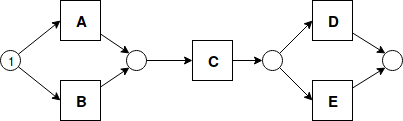
\includegraphics[width=\linewidth]{figures/algorithm/LT_Seq_01_Original.png}
		\caption{The reviewed Petri net}
		\label{fig:pn-lt-demo}
	\end{subfigure}%
\end{figure} 
% here we need to define the long-term dependency
%Based on the concepts above, we give a formal definition for long-term dependency in this thesis. 
%\begin{definition}[Long-term dependency for xor blocks] We call two xor blocks $S=\{X_1,X2,...X_m\}$ and $T=\{Y_1,Y_2,...Yn\}$ with long-term dependency, if 
%	 \[ S \prec T, d  \]
%\end{definition}
\subsubsection{Cases Analysis}
% Here we need to check the combination for all xor branches, but with one example.
There are various types  of long-term dependencies that are able to happen for two xor blocks. To explain those situations better, we define concepts called sources and targets of long-term dependency and then give an example of one Petri net with long-term dependency.
\begin{definition}[Source and target set of long-term dependency]
	The source set of the long-term dependency in two xor blocks is the set of all  xor branches, $LT_S:= \{X \vert \exists Y, X\rightsquigarrow Y  \in LT \} $, and target set is $LT_T:= \{Y \vert \exists X, X\rightsquigarrow Y \in LT \} $. \\
	For one xor branch $X \in S$, the target xor branch set relative to it with long-term dependency is 
	$ LT_T(X)= \{Y \vert  X\rightsquigarrow Y \in LT \}$
	Similarly, the source set related to one target xor branch is
	$ LT_S(Y)= \{X \vert  X\rightsquigarrow Y \in LT \}$
\end{definition}
At the same time, we use $S $ and $T$ to represent the set of xor branches for source and target xor block with long-term dependency.
Given a process tree in Figure \ref{fig:pt-lt-demo}, two xor blocks are contained in the model. They are able to have the following long-term dependencies.
% make it two graphs here, one is the process tree, one is the Petri net.
\begin{enumerate}
	\item $LT=\{ A\rightsquigarrow D, A\rightsquigarrow E, B\rightsquigarrow D, B\rightsquigarrow E\}$. \\
	$LT_S = \{A,B\}, LT_T=\{D,E\}, \vert LT \vert = \vert S \vert * \vert T \vert  $, which is a full long-term dependency where all combinations of source and target xor branches have significant correlation. 
	\item $LT=\{ A\rightsquigarrow D, A\rightsquigarrow E, B\rightsquigarrow E\}. $\\
	$LT_S = \{A,B\}, LT_T=\{D,E\}$
	$LT_S = S $ and $LT_T = T, \vert LT \vert < \vert S \vert * \vert T \vert $. it doesn't cover all combinations. But for one xor branch $X \in S, LT_T(X)= T$, it has all the full long-term dependency with $T$. 
	\item $LT=\{ A\rightsquigarrow D, B\rightsquigarrow E\}. $\\
	$LT_S = \{A,B\}, LT_T=\{D,E\}$
	$LT_S = S $ and $LT_T = T, \vert LT \vert < \vert S \vert * \vert T \vert $. For all xor branch $X \in S, LT_T(X) \subsetneq T$, none of xor branch X has long-term dependency with $T$.
	\item $LT=\{ A\rightsquigarrow D, B\rightsquigarrow D\}.$ \\
	$LT_S = S ,  LT_T \subsetneq T$. There exists at least one xor branch $Y \in T$ which has no long-term dependency on it.
	\item $LT=\{ A\rightsquigarrow D, A\rightsquigarrow E\}.$ \\
	$LT_S \subsetneq S ,  LT_T = T$.
	There exists at least one xor branch in source $X \in S$ which has no long-term dependency on it.
	\item $LT=\{ A\rightsquigarrow E\}. $\\
	$LT_S \subsetneq S ,  LT_T \subsetneq T$.
	There exists at least one xor branch in source $X \in S$  and one xor target xor branch which has no long-term dependency on it.
	\item $ \emptyset$ . There is no long-term dependency on this set. 
\end{enumerate}
% here already to dispose several situations here and then 
%However, when the long-term dependency is full connected where each combination of xor branches from source and target xor block has long-term dependency, namely xor branches can be chosen freely, we don't add any places and silent transitions on the model.
In the listed situations, situation 1 is a full long-term dependency, which allows all combinations like the original models, and no changes is necessary on the model. Situation 7 has no long-term dependency, where the correlation of them is either not so strong from the positive instances or rejected from negative instances. In this thesis, we don't take those two situations into consideration.  

%% should we write down here to prove the correctness of available situations, or we need to wait??
\subsubsection{Way to Express Long-term Dependency}
% but how to come from the process tree to Petri net??? 
After detecting long-term dependencies with xor branches in process tree, it is not possible to express those dependencies on process tree by using the current process tree operators. Moreover, the final output of our task demands a Petri net. Therefore, we convert the generated process tree into a Petri net and express long-term dependency on the Petri net with corresponding structures.

According to \cite{bergenthum2007process}, adding places to transitions in Petri net can limit the model behavior. Any transition demands a token from its input places to fire. When there is no token at this place, the transitions are not enabled. By adding extra places to the Petri net, it can block negative behaviors which are not expected in the aspect of business performance. 

Long-term dependency limits the available choices to fire transitions after the previous xor branch executes. So to express long-term dependency, our basic idea is to add places connected to transitions in the Petri net. In addition, because one xor branch can be as a source to multiple long-term dependencies and one xor branch can be as a target to multiple long-term dependencies, silent transitions are also needed to explicitly address a long-term dependency. 


Firstly, the long-term dependency set from process tree is mapped to the corresponding Petri net. For an arbitrary long-term dependency set $LT=\{X_i \rightsquigarrow Y_j \vert 1 \leq i \leq m, 1 \leq j \leq n \}$ with $S=\{X_1,X2,...X_m\}$ and $T=\{Y_1,Y_2,...Yn\}$ in Petri net, we add places after the source xor branches in Petri net,  $P_S=\{p_{X_i} \vert X_i \in LT_{S} \}$, and places before target xor branches,$P_T=\{p_{Y_j} \vert Y_i \in LT_{T} \}$. For each long-term dependency $X_{i} \rightsquigarrow Y_{j}$ in LT, there is silent transition t with $p_{X_i} \rightarrow t \rightarrow p_{Y_{j}}$. The steps to add silent transitions and places according to the long-term dependency are listed in algorithm \ref{alg: Adding method}.

% An algorithm is given to show how to add the long-term dependency
\begin{algorithm}[!ht]
	\SetAlgoLined
	$Y$ is dependent on $X$\;
	\If{$X$ is leaf node}{
		One place is added after this leaf node \;
	}
	\If{$X$ is Seq}{
		Add a place after  the end node of this branch\;
		The node points to the new place\;
	}
	\If{$X$ is And}{
		Create a place after the end node of every children branch in this And xor branch \; 
		Combine all the places by a silent transition after those places \;
		Create a new place directly after silent transition to represent the And xor branch \;
	}
	
	\If{$Y$ is leaf node}{
		One place is added before this leaf node \;
	}\If{$Y$ is Seq}{
		Add a place before  the end node of this branch\;
		The new place points to this end node\;
	}\If{$Y$ is And}{
		Create a place before the end node of every children branch in this And xor branch \; 
		Combine all the places by a silent transition before those places \;
		Create a new place directly before silent transition to represent the And xor branch \;
	}
	Connect the places which represent the $X$ and $Y$ by creating a silent transition.
	\caption{Add long-term dependency between pure xor branch}
	\label{alg: Adding method}
\end{algorithm}
\begin{figure}
	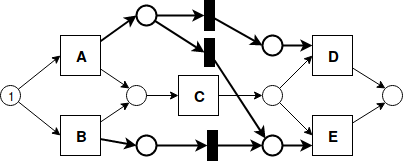
\includegraphics[width=\textwidth]{figures/algorithm/LT_Seq_01_Silent_01.png}
	\caption[Model with long-term dependency]{Model with long-term dependency $LT=\{ A\rightsquigarrow D, A\rightsquigarrow E, B\rightsquigarrow E\}. $ }
	\label{fig:pn-demo-with-lt}
\end{figure}
Reviewing the example of process tree of Figure \ref{fig:pt-lt-demo}, it has long-term dependency set $LT=\{ A\rightsquigarrow D, A\rightsquigarrow E, B\rightsquigarrow E\}$. To express long-term dependency,  the process tree is firstly transformed into the Petri net as Figure \ref{fig:pn-lt-demo}. Then two extra places are added respectively after A and B; Next, two places before D and E are created to express that the xor branches are involved with long-term dependency. At end, for each long-term dependency, a silent transition is generated to connect the extra places after the source xor branch to the place before target place. The generated model with long-term dependency is displayed in Figure \ref{fig:pn-demo-with-lt}.

\subsubsection{Soundness Analysis}
% this section is used to select the sound situations. 
% next time I can go to library at Tuesday with the laptop and study there..
With Algorithm \ref{alg: Adding method} by adding silent transitions and places to express long-term dependency, the model soundness can be violated. In the following section, we discuss the soundness in different situations. 

Given a Petri net with long-term dependency $LT=\{X_i \rightsquigarrow Y_j \vert 1 \leq i \leq m, 1 \leq j \leq n \}$ on two xor blocks $S=\{X_1,X2,...X_m\}$ and $T=\{Y_1,Y_2,...Yn\}$. After applying the Algorithm \ref{alg: Adding method}, $P_S=\{p_{X_i} \vert X_i \in LT_{S} \}$ , $P_T=\{p_{Y_j} \vert Y_i \in LT_{T} \}$, and silent transitions $ E = \{\epsilon \vert p_{X_i} \rightarrow \epsilon
\rightarrow p_{Y_{j}} \}$ are added. 
 
The Petri net is sound if and only if (1)the soundness outside xor blocks with long-term dependency is not violated; and  (2) soundness between xor blocks is kept. In the following, we check the model soundness with long-term dependency after applying Algorithm \ref{alg: Adding method}. \\\\
\textbf{Soundness outside xor blocks.}\\
	\emph{Proof:} he added silent transitions and places do not violate the execution outside of the xor blocks, because the extra tokens that are generated due to long-term dependency are constrained in the xor blocks, and it doesn't affect the token flows outside. As we know, the original model is sound. So the soundness outside xor blocks is not violated.
%% begin to prove the soundness inside xor block
\\\\
\textbf{Soundness inside xor blocks.}\\
For the xor blocks $S=\{X_1,X2,...X_m\}$ and $T=\{Y_1,Y_2,...Yn\}$ with long-term dependency $LT=\{X_i \rightsquigarrow Y_j \vert 1 \leq i \leq m, 1 \leq j \leq n \}$, only one xor branch can be fired in S. Without loss of generality, $X_i$ is assumed to be enabled. After firing $X_i$, the marking distribution on the extra places are  
\[ M(p_{X_i}) = 1; \quad 
\forall p_{X_i^\prime} \in P_S, i^\prime \neq i, M(p_{X_i^\prime})=0 \]
%% here we need to divide them into different situations...
If $ LT_S = S, LT_T=T$, adding the long-term dependency in this situation doesn't violate the model soundness, we prove it in the following part.
%the following conditions are checked. 
\begin{itemize}
	\item Safeness. Places cannot hold multiple tokens at the same time.\\
	For all extra places $p_{X_i}$ and $p_{Y_j}$, 
	\[\forall p_{X_i} \in P_S, \sum M(p_{X_i})=1\]
	Because $ LT_S = S, X_i \in S$, so $X_i \in LT_S$, there exists one $Y_j$ with $X_i \rightarrow Y_j$ and one $\epsilon, p_{X_i} \rightarrow \epsilon
	\rightarrow p_{Y_{j}} $.  After firing $X_i$, the transition $\epsilon$ becomes enable. After executing $\epsilon$, the marking distribution turns to 
	\[ M(p_{Y_j}) = 1;\quad 
	\forall p_{Y_j^\prime} \in P_T, j^\prime \neq j,  M(p_{Y_i})=0 \]
	So whenever the marking distribution in the extra places are
	\[\sum M(p_{X_i}) \leq 1,  \sum M(p_{Y_j}) \leq 1 \] 
	\item Proper completion. If the sink place is marked, all other places are empty. \\
	After firing $Y_j$, all the extra places hold no token. So it does not violate the proper completion.
	\item Option to complete.  It is always possible to reach the final marking just for the sink place. \\
	There is always one $Y_j$ enabled after firing $X_i$ to continue the subsequent execution.
	\item No dead part. For any transition there is a path from source to sink place. \\
	Because all $Y_j \in T$ are also in $LT_T$, there exists at least one $X_i\in S$ with long-term dependency with $Y_j$. After $X_i$ is fired, one token is generated on the extra place $p_{X_i}$ and can be consumed by silent transition $\epsilon$ in  $p_{X_i} \rightarrow \epsilon \rightarrow p_{Y_{j}}$ to produce a token in $p_{Y_j}$, which enables xor branch $Y_j$ and leaves no dead part.
\end{itemize}
In other situation, the model becomes unsound. \\
\indent If $LT_S \neq S,or\quad LT_T \neq \emptyset$, there exists one xor branch $X_i$ with $X_i \notin LT_S$. When $X_i$ is fired, it generates one token at place $p_{X_i}$, this token cannot be consumed by any $Y_j$. So it violates the proper completion. \\  
\indent If $LT_T \neq T$, there exists one $Y_j \notin LT_T, \nexists X_i, X_i \rightsquigarrow Y_j$, so with two input places but $Token(p_{Y_j})=0$,  $Y_j$ becomes the dead part, which violates the soundness again. 
As a conclusion, to keep Petri net with long-term dependency sound, only situations with $ LT_S = S, LT_T=T$ are considered.  
\subsection{Reduce Silent Transitions}
%% We reduce the silent transition when there is no 
Our method to represent long-term dependency can introduce redundant silent transitions and places, which complicates the model. So, we post process the Petri net with long-term dependency and delete redundant silent transitions and places in it. 
% definition of redundant transitions and places
Silent transitions and places of a Petri net are redundant when the Petri net preserves the behavior without those transitions and places \cite{murata1989petri, verbeek2017decomposed}. There is an existing algorithm developed in work of \cite{verbeek2017decomposed}. We reuse it as one post procedure in our thesis. 

%% here we need to prove this proposition
One example is given in the following graph. $M_{lt}$ in Figure \ref{fig:with-lt} has long-term dependency expressed in the silent transitions and places. The silent transition for $S2 \rightsquigarrow B1 $ and silent transition for $B1 \rightsquigarrow T2$ belongs to the case (1). So they are kept in the model, while the other silent transitions are deleted. After reducing the redundant silent transitions, the model becomes $M_r$ shown in Figure \ref{fig:reduced-lt}. Those two models have the same behavior, yet the reduced model is simpler.
\begin{figure}[!h]
	\centering
	\begin{subfigure}[a]{\textwidth}
		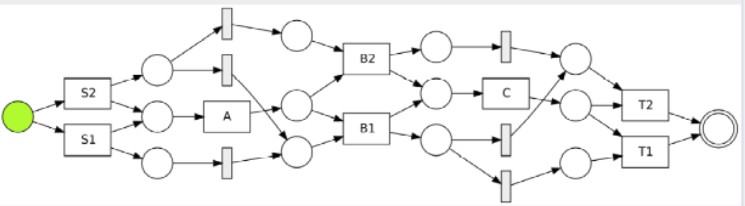
\includegraphics[width=\textwidth]{figures/algorithm/dfg-IM-pn-with-lt.png}
		
		\caption{A Petri net $M_{lt}$ with redundant silent transitions}
		\label{fig:with-lt}
	\end{subfigure}
	\hfill
	\begin{subfigure}[b]{\textwidth}
		\centering
		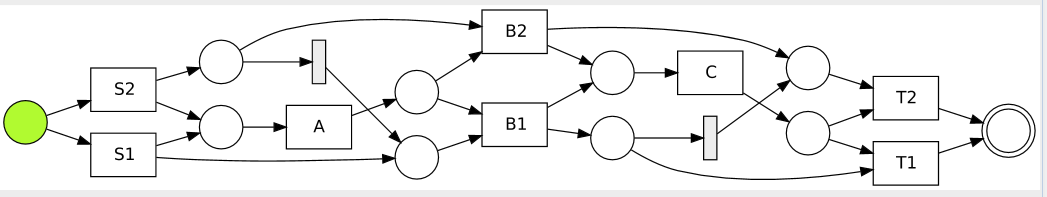
\includegraphics[width=\linewidth]{figures/algorithm/dfg-IM-pn-with-lt-reduced.png}
		
		\caption{Petri net $M_r$ with reduced silent transitions}
		\label{fig:reduced-lt}
	\end{subfigure}
\end{figure}
\subsection{Concrete Architecture}
At last, we assemble all the modules together and give an overview architecture of our repair techniques.  We reuse existing modules in gray rectangles in Figure \ref{fig:architecture}, e.g. IMLog2Dfg to convert an event log into directly-follow graph, Petrinet2TransitionSystem to transform a Petri net into a transition system. The other modules are programmed according to our specific needs and achieve the repair algorithm mentioned before. To achieve a preciser Petri net, the module to add long-term dependency becomes a necessary part. Yet, reduction on redundant places and silent transitions is optional. 
\begin{figure}
	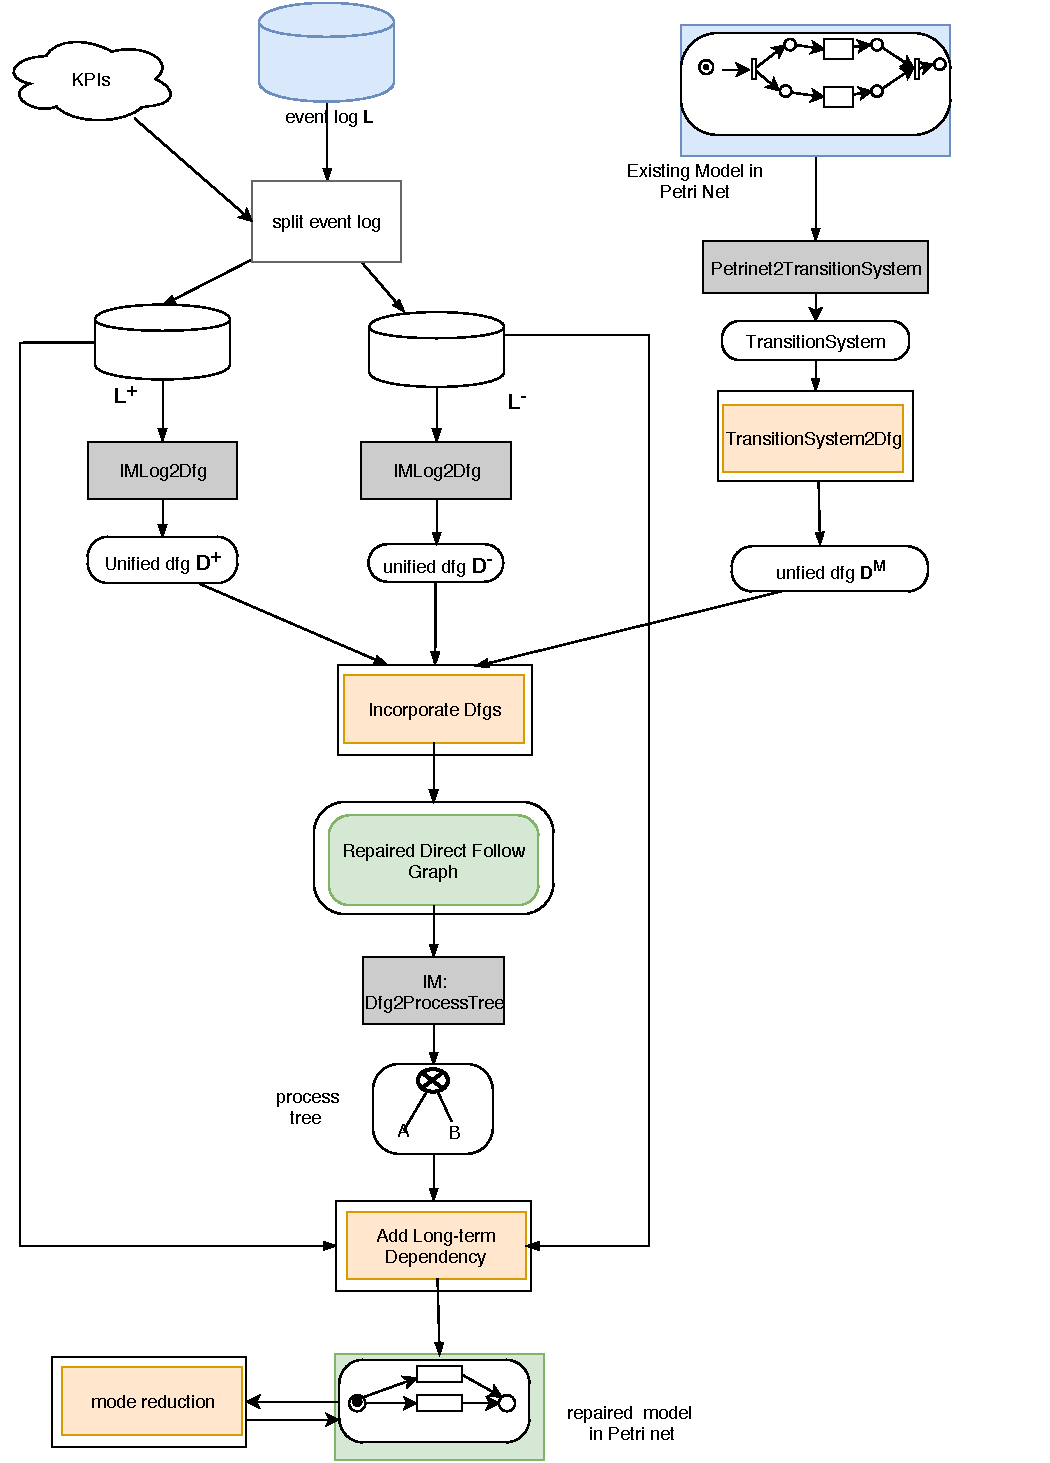
\includegraphics[height=0.9\textheight]{figures/algorithm/FD_architeccture_details.pdf}
	\caption[Model Repair Architecture]{Model Repair Architecture -- \small Rectangles represents processes and output data in eclipse shape, especially customized processes and data are in doubled lattice shape. Input event log and existing model are in blue, KPIs are in cloud. The output is a petri net in purple.}
	\label{fig:architecture}
\end{figure} 


\chapter{Implementation} \label{chap:impl}
%%This chapter is used to show our implementation in ProM.  It can be split into 3 parts. 
%The first one is the Dfg method, including the weight update, process tree generation and petri net without long-term dependency generation.
% The second part is to add long-term dependency, it can be use as whole part or customized part into model, also removing the long-term dependency
% Evaluation part is the confusion matrix measurement.
%% Change implementation structure in this way::
%% 1. platform introduction, ProM + KNIME platforms
%% 2. No neccessary to describe the input right?? Aslo, there are another new concepts shown in the graph, which we need to avoid it. 
%% 3. then the screenshots to show the steps of the implementation
%% 4. If we introduce the property here, really, it will not help.. In this way, it can be fine.. But just add the introduction part for the KNIME
In this chapter, we begin with the introduction of implementation platforms for our methods and then show the use of those applications step by step.

\section{Implementation Platforms}
\subsection{Process Mining Platform -- ProM}
ProM is an open-source process mining tool in Java that is extensible by adding a set of plug-ins \cite{ProM}. ProM supports a wide variety of process mining techniques and is usually used for academic research. We implement the algorithm on ProM 6.8, which is the latest stable version. The corresponding plugin is \textbf{\emph{Repair Model By Kefang}} and released online \cite{MyPlugin}.

\subsection{KNIME}
KNIME Analytics Platform is an open-source software to help researchers analyze data. Multiple modules are integrated into this platform for loading, transforming and processing data. Researchers can achieve their goals by creating visual workflows composed of expected modules implemented as nodes with an intuitive, drag and drop style graphical interface, rather than focusing on any particular application area.

The reasons to integrate our techniques into KNIME are (1)KNIME is widely used in scientific research and benefits the application of our techniques;(2)KNIME supports automation of test workflow, which helps conduct more efficient experiments.  However, the integration requires additional development effort.
% here we need to change the name of our sections, because if we present them into a general way, so we need to show them in a general methods.
\section{Generate a Petri net}
Firstly two dialogs are poped up to set the arguments, such as the event classifier to  generate directly-follows graphs from event logs. Subsequently, a dialog is shown to set the Inductive Miner parameters. The parameters include the Inductive Miner variant and the noise threshold to filter the data. The dialog is displayed in Figure \ref{fig:dfg-IM-setting}.
\begin{figure}
	\centering
	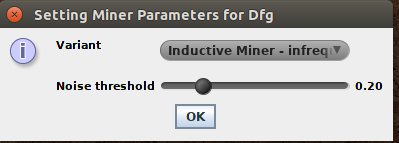
\includegraphics[scale=0.75]{figures/implementation/dfg-IM-setting.png}
	\caption{Inductive Miner Parameter Setting}
	\label{fig:dfg-IM-setting}
\end{figure} \\
After setting the parameters, process models  of process tree and Petri net without long-term dependency can be generated by Inductive Miner and displayed in the result view in Figure \ref{fig:dfg-IM-pn-without-lt}. 
\begin{figure}
	\centering
	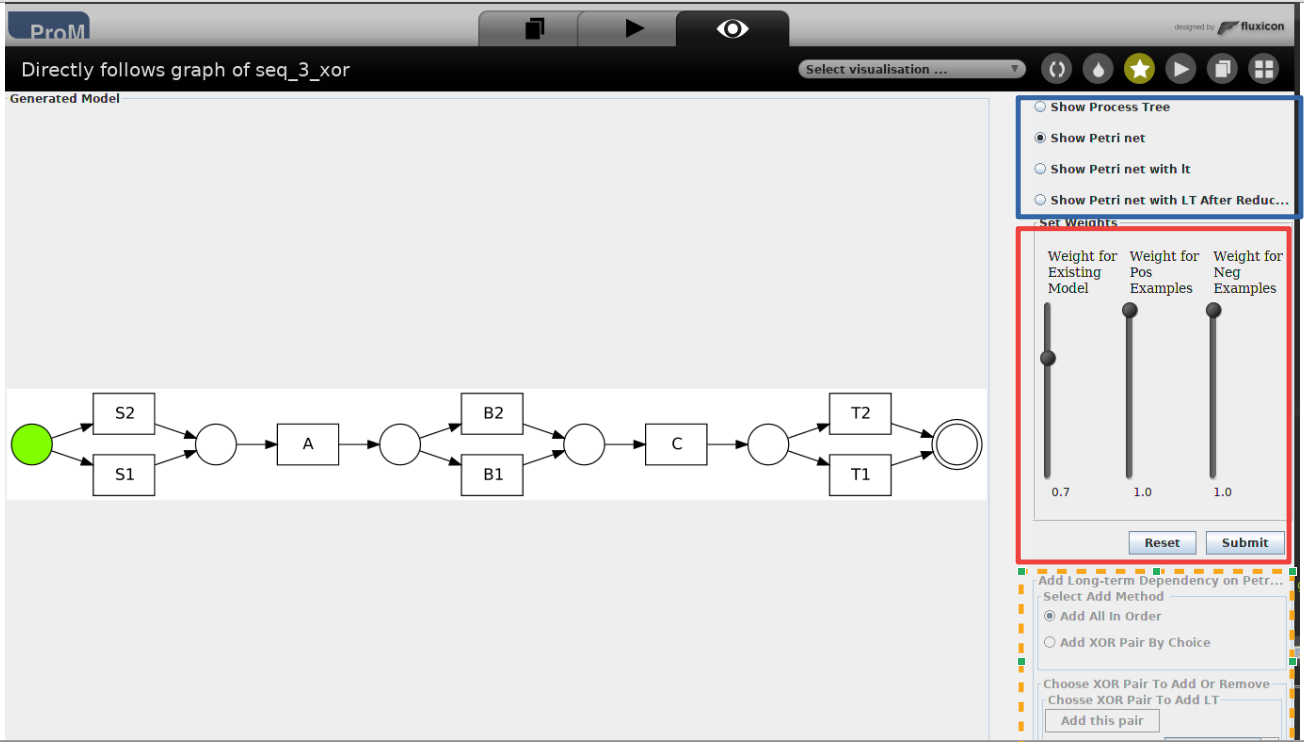
\includegraphics[width=\textwidth]{figures/implementation/dfg-IM-pn-without-lt.png}
	\caption{Generated Petri net without long-term dependency}
	\label{fig:dfg-IM-pn-without-lt}
\end{figure}
The left side is the model display area, where the right panel is to set the control parameters for the existing model, positive or negative instances. In interactive way, more flexibility is allowed by this plug-in to repair model. By default, the generated model type and the weight sliders are enabled at first. The control panel for adding long-term dependency are only triggered after choosing the option to repair model with long-term dependency. 

The model type is selected in the blue rectangle marked in Figure \ref{fig:dfg-IM-pn-without-lt}. It has 4 options to control the generated model type. Currently, the option "Show Petri net" is chosen, so the constructed model is Petri net without long-term dependency. The weights sliders are in red rectangle. They adjust the weights for the existing model, positive and negative instances. Once those options are submitted, different process models are mined under different weights. The rectangle in orange are the invisible part to control long-term dependency options. It will be discussed in the next section.

\section{Post Process to Add Long-term Dependency }
If we want to repair the Petri net with long-term dependency, one post procedure is triggered to add long-term dependency . This program in the background detects and puts places and silent transitions on Petri net directly mined from Inductive Miner to add long-term dependency. As comparison, the same weight setting is kept like the Figure \ref{fig:dfg-IM-pn-without-lt}, but the option to show a Petri net with long-term dependency is chosen. The resulted model is displayed in  Figure \ref{fig:dfg-IM-pn-with-lt}. 
\begin{figure}
	\centering
	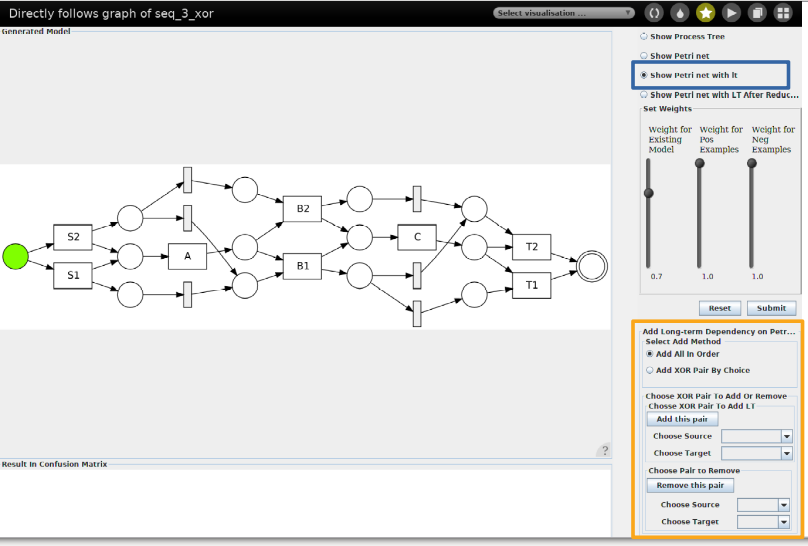
\includegraphics[width=\textwidth]{figures/implementation/dfg-IM-pn-with-lt.png}
	\caption{Petri Net with long-term dependency }
	\label{fig:dfg-IM-pn-with-lt}
\end{figure}

Meanwhile, the control part of adding long-term dependency turns visible in the orange rectangle like in Figure \ref{fig:dfg-IM-pn-with-lt}.  It has two main options, one is to consider all long-term dependencies existing in the model, the other is to choose the part manually. It allows more flexibility for users. Below those two options are the manual selection panels, including a control part to add and remove pair. As an example, the blocks Xor(S1,S2) and Xor(T1,T2) are chosen to add long-term dependency. It results in the model in Figure \ref{fig:dfg-IM-pn-with-lt-m}. 
\begin{figure}[h]
	\centering
	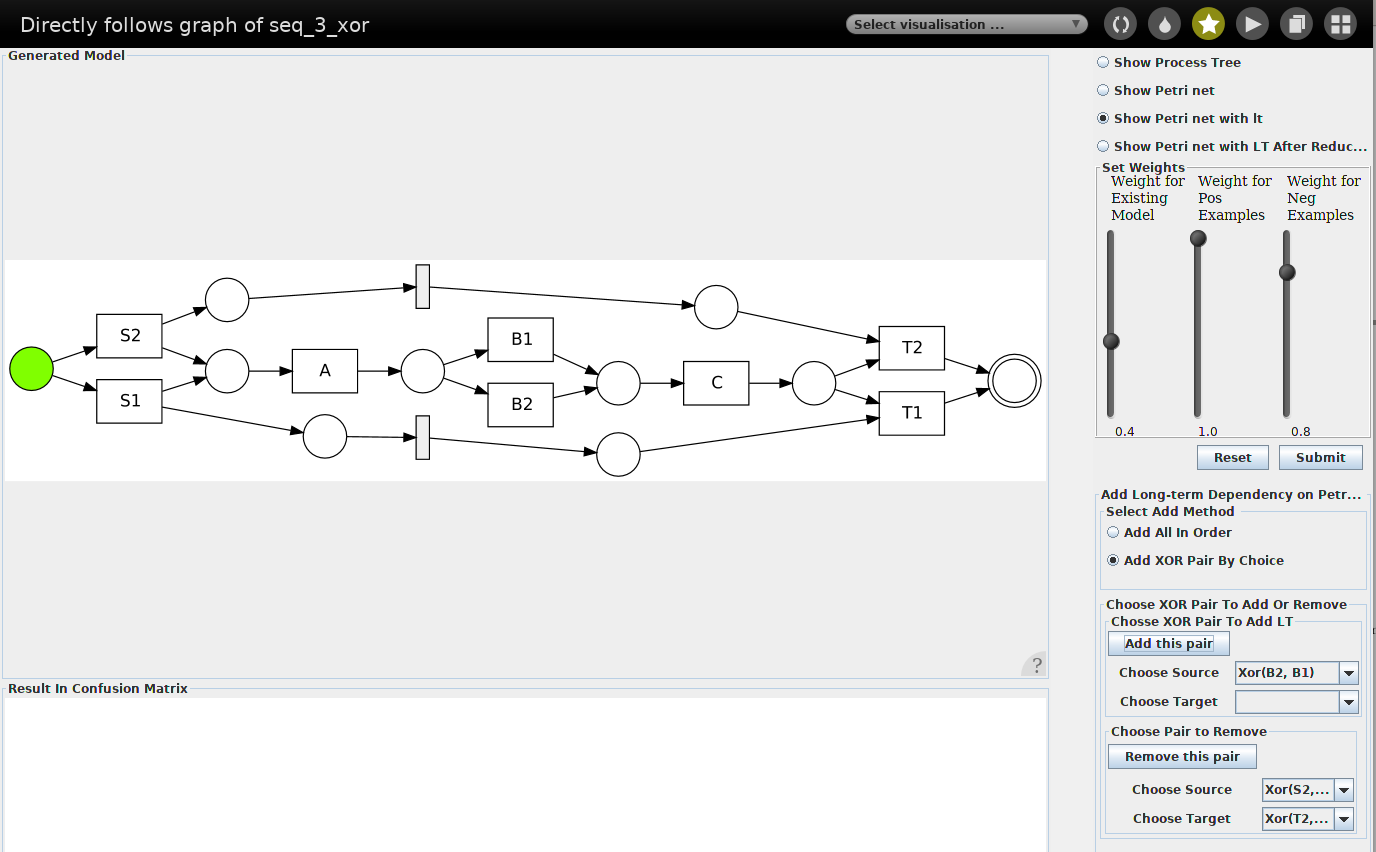
\includegraphics[width=\textwidth]{figures/implementation/dfg-IM-pn-with-lt-manual.png}
	\caption{Petri net with selected long-term dependency}
	\label{fig:dfg-IM-pn-with-lt-m}
\end{figure}
\section{Post Process to Reduce Redundant Silent Transitions and Places}
By choosing the option of \emph{Petri net with LT After Reducing} in model type, silent transitions and places are reduced to simplify the model.
Under the same setting in Figure \ref{fig:dfg-IM-pn-without-lt}, the simpler model in Figure \ref{fig:dfg-IM-pn-with-lt-r} is constructed, after the post processing of reducing silent transitions.
\begin{figure}[h]
	\centering
	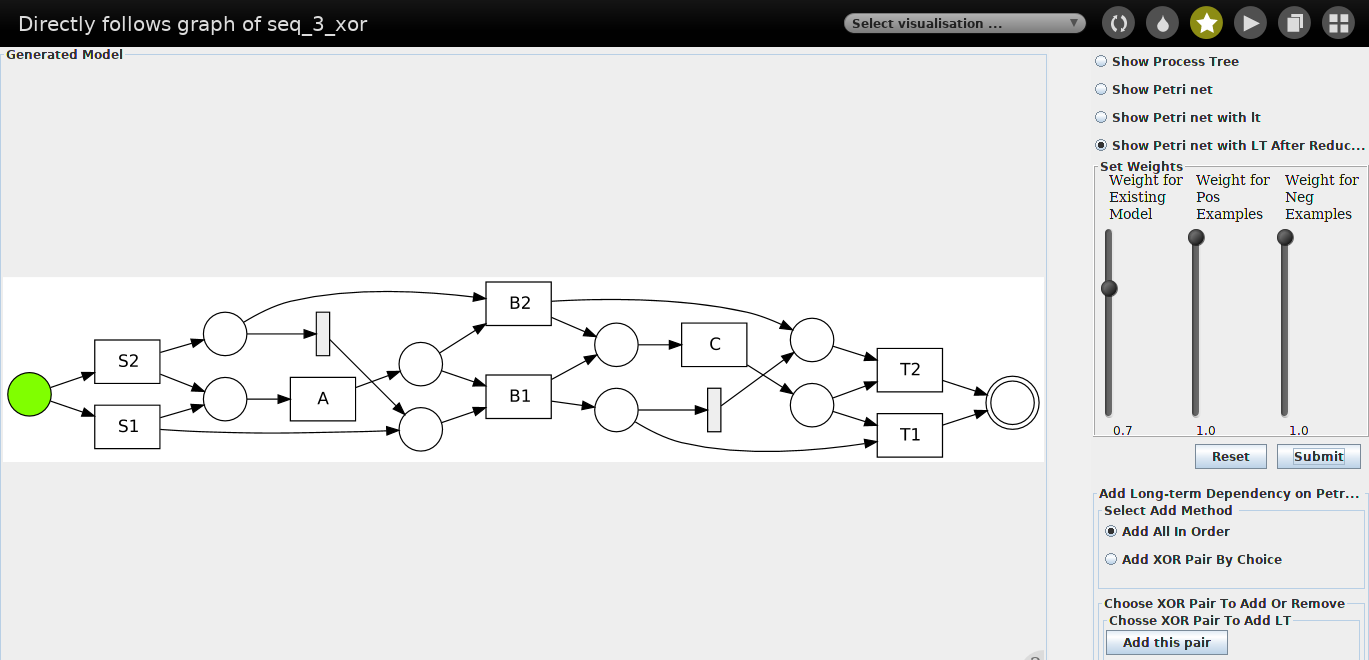
\includegraphics[width=\textwidth]{figures/implementation/dfg-IM-pn-with-lt-reduced.png}
	\caption{Petri net after reducing the silent transitions}
	\label{fig:dfg-IM-pn-with-lt-r}
\end{figure}

\section{Additional Feature to Show Evaluation Result}
Another feature in this plugin  is to show the evaluation result based on confusion matrix. With the brief evaluation result, it helps set the parameters for the optimal Petri net. 

After creating the current model in the left view, the evaluation program in background uses the event log and the current Petri net in the view as inputs. A naive fitness checking is applied on the repaired model with the event log. This procedure is based on the existing plugin in ProM -- \textbf{PNetReplayer}. This plugin checks if the trace fits the model and give out the one possible deviation with minimal cost. In our implementation, either the deviation on model or in trace is set with the same cost. Based on the deviation result and the label information on each trace, a confusion matrix is generated. Moreover, relative measurements like recall, precision are calculated and shown in the bottom of the left view in Figure \ref{fig:dfg-IM-cm}.  If the button of green rectangle in the right view \emph{Show Confusion Matrix} is pressed again, the program is triggered again and generates a new  confusion matrix result in the dark green dashed rectangle which will be listed above the previous result in light green dashes area. 
\begin{figure}
	\centering
	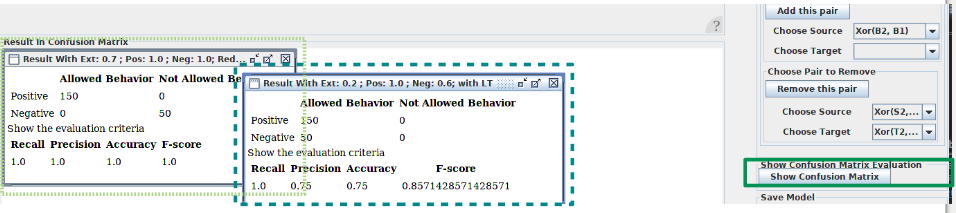
\includegraphics[width=\textwidth]{figures/implementation/dfg-IM-confusionmatrix.png}
	\caption{Generated Process Tree Model}
	\label{fig:dfg-IM-cm}
\end{figure}

\section{Integration into KNIME}
% this section describes the integration of our algorithm with KNIME, should we introduce some parts abotu them?? Yes, here about our real implementation, above should introduce the basic implementation steps.
\emph{Nodes} in the workflow represents different modules corresponding the plugins in ProM. Each node has certain input ports on the left side to represent the required parameters and  ports on the right to output result. By connecting the ports between nodes, data are passed and processed by one node after another. To integrate our algorithm into KNIME, other related modules on process mining are necessary, which can be divided into the following categories: 
% make a lot of work here to express your work
\begin{enumerate}
	\item Data importer and exporter. The importers and exporters for event logs, process trees and Petri nets are implemented to load and save basic data for Process Mining.
	\item Event logs manipulation. Nodes for splitting, sampling and assigning labels to event logs are implemented to benefit our experiments.
	\item Classic discovery algorithms. Inductive Miner and Alpha Miner are integrated into KNIME to provide baselines for our algorithm.
	\item Model enhancement. Our proposed method is integrated in KNIME to repair model in Petri net.
\end{enumerate}

To integrate our repair algorithm from ProM into KNIME, we need to create the workflow in the Figure \ref{fig:impl-KNIME}. After reading a Petri net by  \emph{PetrinetReader} and an event log by \emph{Import Event Log(XES)}, Node \emph{IncorporateNegInfo} applies the algorithm in this thesis to repair a model in Petri net with incorporating negative information. The outputs have different kinds of Petri nets to match the ones generated in ProM, eg. reduced Petri net with long-term dependency, Petri net without long-term dependency. In addition, we can evaluate our repaired model by using the node \emph{RepairEvaluator}. At last, we can save the repaired Petri net by \emph{PetrinetWriter}.
% give a screen shot and list the explaination on it.
\begin{figure}
	\centering
	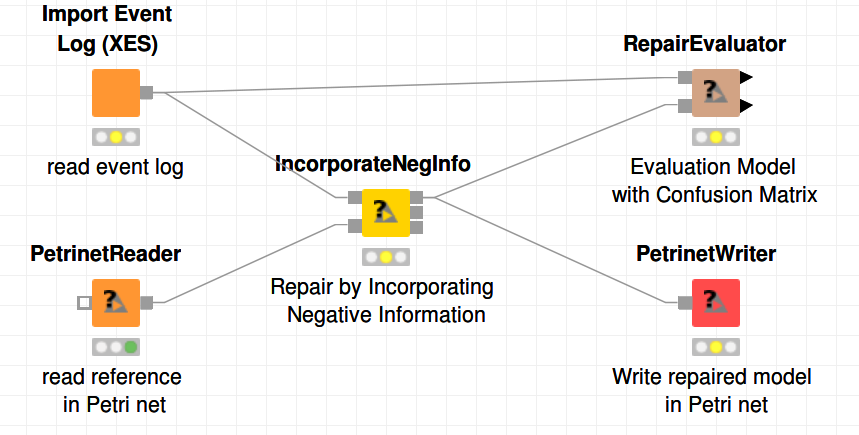
\includegraphics[width=\textwidth]{figures/implementation/implementation-KNIME.png}
	\caption{Integration of our repair techniques into KNIME}
	\label{fig:impl-KNIME}
\end{figure}

\fi
\chapter{Evaluation} \label{chap:eval}
%%This is the evaluation part, int includes the following parts.
% <1> Evaluation Metrics, explain the measurements chosen for this experiments
% <2> Test Platform in KNIME, introduced before so we don't really need to repeat it here
% Firstly, we validate our methods and make sure it works for the properties.. Then using the whole data to test the weights tend and also, if it handled the real life data. 
% <3.1> validation part to check the methods work for those situations, but not necessary;; Then big data test to show property to handle those situations. 
% <3> Test Cases Design, the parameters we want to compare, the cases
%   ==> synthetic data
%   ==> Real life data
%   ++ Data to test the property
This chapter presents an experimental evaluation of our repair techniques. At first, we define the evaluation criteria. Next, we briefly introduce the test platforms KNIME and relevant ProM plugins tools. Then, we conduct two kinds of tests. One is based one the demo example proposed in the introduction part, one is on the real life data. 
\section{Evaluation Measurements}
% First talk about our data and our model, then choose the confusion matrix as one measurements. But we should review the traditional measuremtns on process mining before introducing the confusion matrix. but we should also focus on the accuracy part and f-score.
We evaluate repair techniques based on the quality of repaired models with respect to the given event logs. In process mining, there are four quality dimensions generally used to compare the process models with event logs. 
\begin{itemize}
	\item \emph{fitness.} It quantifies the extent of a model to reproduce the traces recorded in an event log which is used to build the model. Alignment-based fitness computation aligns as many events from trace with the model execution as possible.  
	\item \emph{precision.} It assesses the extent how the discovered model limits the completely unrelated behavior that doesn't show in the event log. 
	\item \emph{generalization.} It addresses the over-fitting problem when a model strictly matches to only seen behavior but is unable to generalize the example behavior seen in the event log. 
	\item \emph{simplicity.} This dimension captures the model complexity. According to Occam's razor principle, the model should be as simple as possible.
\end{itemize}
% How to come to confusion matrix?? 
The four traditional quality criteria are proposed in semi-positive environment where only positive instances are available. Therefore, when it comes to the model performance, where negative instances are also possible, the measurement metrics should be adjusted. With labeled traces in the event log, the repaired model can be seen as a binary prediction model where the positive instances are supported while the negative ones are rejected. Consequently, the model evaluation becomes a classifier evaluation. 

% Describe its features and some derived measurements. 
Confusion matrix has a long history to evaluate the performance of a  classification model. A confusion matrix is a table with columns to describe the prediction model and rows for actual classification on data.  The repaired model can be seen a binary classifier and produces four outcomes- true positive, true negative, false positive and false negative shown in the Table \ref{tab:cm}.
\begin{itemize}
	\item True Positive(TP): The execution allowed by the process model has an positive performance outcome.
	\item True Negative(TN): The negative instance is also blocked by the process model.
	\item False Positive(FP): The execution allowed by the process model has an negative performance outcome.
	\item False Negative(FN):The negative instance is enabled by the process model.
\end{itemize} 
% confusion matrix
\begin{table}[]
	\caption{Confusion Matrix}
	\label{tab:cm}
	\begin{tabular}{ll|c|c|}
		\cline{3-4}
		&                   & \multicolumn{2}{c|}{repaired model}                                               \\ \cline{2-4} 
		\multicolumn{1}{l|}{}                                                                         &                   & \multicolumn{1}{l|}{allowed behavior} & \multicolumn{1}{l|}{not allowed behavior} \\ \hline
		\multicolumn{1}{|l|}{\multirow{2}{*}{\begin{tabular}[c]{@{}l@{}}actual \\ data\end{tabular}}} & positive instance & TP                                    & FN                                        \\ \cline{2-4} 
		\multicolumn{1}{|l|}{}                                                                        & negative instance & FP                                    & TN                                        \\ \hline
	\end{tabular}
\end{table}
Various measurements can be derived from confusion matrix. According to our model, we choose the following ones as the potential measurements. 
\begin{itemize}
	\item recall. It represents the true positive rate and is calculated as the number of correct positive predictions divided by the total number of positives.
	\[Recall = \frac{TP}{TP + FN}\]
	\item precision. It describes the ability of the repaired model to produce positive instances.
	\[Precision = \frac{TP}{TP + FP }\]
	%\item specificity. In opposite with recall, it measures the true negative rate.
	%\[Specificity = \frac{TN}{TN + FP}\]
	\item accuracy. It is the proportion of true result among the total number. It  measures in our case how well a model correctly allows the positive instances or disallows the negative instances.
	\[Accuracy = \frac{TP+TN}{TP+TN+FP+FN}\]
	\item F-score is is the harmonic mean of precision and recall.
	\[F_1 = \frac{2*Recall*Precision}{Precision + Recall}\]
\end{itemize}
Generally, there is a trade-off between the quality criteria. So the measurements are only used to compare specific aspects of our techniques.
\section{Experiment Platforms}
KNIME, as a scientific workflow analytic platform, supports automation of test workflow, which helps us repeat experiments efficiently. Yet, traditional evaluation plugins in ProM are not integrated into KNIME, so partial experiments are conducted in ProM.
\subsection{KNIME}
% this section describes how KNIME supports automatic test, FlowVariable and optimization parts of it.
KNIME supports automation of test workflow mainly through the following mechanisms. 
\begin{itemize}
	\item Loop Control Structure. KNIME provides a bunch of control nodes which support re-executing workflow parts.  Nodes representing \emph{Loop Start} appear in pairs with nodes for \emph{Loop Nodes}, the workflow between pairs is executed recursively in a fixed number, or until certain conditions are met. In our test, we repeat our repair techniques for different parameter settings by applying loop structure into KNIME workflow.
	\item Flow Variables. Flow Variables are used inside a KNIME workflow to parameter node settings dynamically. When it combines with loop control structure, tests with different settings is able to conduct automatically.
\end{itemize}
What's more, there are nodes provided by KNIME to optimize the value of some parameters with respect to a cost function. As long as a cost function is provides, KNIME is able to automatically optimize any kind of parameters. 
\subsection{ProM Evaluation Plugins}
%Here we discuss the plugins to test other aspects of our methods. 
Although KNIME offers a powerful approach to conduct experiments, the integration of traditional process mining evaluation plugins into KNIME is out of our capability due to the time limits. To evaluate repaired models with traditional metrics, we use an existing ProM plugin called \textbf{\emph{Multi-perspective Process Explorer}} \cite{mannhardt2015multi}. This plugin accepts  Petri net and an event log as inputs, and gives out fitness, and precision measurements which are based on the traditional alignment conformance checking. 
\section{Experiment Results}
\subsection{Test on Demo Example}
In this experiment, we aim to answer the question: Will our repair method overcome shortcomings of current techniques which are shown in the introduction chapter?  

% for situation 1, we can not get the ideal model, the reason is that we can not keep the model like just as it states, we can 

\subsection{Comparison To Other Techniques}
This section represents some situations where current repair techniques can't handle properly, while our algorithm gives out an improved repaired model. 

\emph{Situation 1}, unfit part!! added subprocess are too much!! Where the addition of subprocesses and loops are allowed, while the structure changes are impossible, 
Fahrland's method applies the extension strategy to repair model by adding subprocesses and loops in the procedure. It introduces unseen behavior into the model. However, if the behaviors which are already in the model is unlikely to be removed from the model. One simple example is shown in the following part. 

Dee's method is based on Fahrland's method. Deviations are calculated at first and used to build subprocesses for model repair. However, before building subprocesses, it classifies the deviations into positive and negative ones with consideration of trace performance. Only positive deviations are applied to repair model. Different to Fahrland's method, it improves the repaired model performance by limiting the introduced subprocesses. Still, it can't get rid of the defect mentioned before. 

\emph{Situation 2}, For fitted data in the model, can not recognize them!! where overlapped data noise can not be recognized, trace variant with more negative effect is treated as positive and kept in the model, which we should delete them.   
% Here we want to give an example of the overlapped data, compared to IM rediscoverty, easy.. But for Dees' method, firstly, they have labeled data; The analyzed the deviations of them, but when one deviation dominates, then the tree can not see the others. Some data are ignored..

\emph{Situation 3}, with long-term dependency!! fitted part or new added part!! none of the current techniques can handle this problem yet.
Simple examples listed, but will this repeat the last section?? 


% Conclusion part
For one exclusive choices, 
but with long-term dependency detected and added in the model, precision and accuracy increase, since model with long-term dependency blocks the negative information by adding transitions and places to limit activity selection. 

\subsection{Test On Real life Data}
% here we will list all the data here but before describe the test data
\subsubsection{Data Description}
\subsubsection{Test Result}
% we don't need to transfer page to landscape view, because we have many rows too.
	\begin{table}[]
		\centering
		\caption{Test Result on BPI15-M1 data}
		\resizebox{\textwidth}{!}{
		\begin{tabular}{lll|llllllll|ll}
			\hline
			\multirow{2}{*}{\thead{event \\ log}} & \multirow{2}{*}{\thead{reference \\ model} }                &    \multirow{2}{*}{\thead{method}}       & \multicolumn{8}{l}{ \thead{confusion matrix metrics}}                              & \multicolumn{2}{|l}{\thead{traditional metrics}} \\
			\cline{4-13}
			 &  &     &
			  \thead{TP}  & \thead{FP} & \thead{TN}  & \thead{FN}  & \thead{recall} & \thead{precision} & \thead{accuracy} & \thead{F1}   & \thead{fitness}           & \thead{precision}           \\
			  \hline
			D1.1      & M1              & IM & 137 & 48 & 118 & 289 & 0.32   & 0.74      & 0.43     & 0.45 & ?                 & ?                   \\
			D1.1      & M1              & Fahland   & 0   & 0  &     &     &        &           &          &      &                   &                     \\
			D1.3      & M1              & Dees      &     &    &     &     &        &           &          &      &                   &                     \\
			D1.3      & M1              & dfg       &     &    &     &     &        &           &          &      &                   &                     \\
			D1.1      & M2              & IM  &     &    &     &     &        &           &          &      &                   &                     \\
			D1.1      & M2              & Fahland   &     &    &     &     &        &           &          &      &                   &                     \\
			D1.3      & M2              & Dees      &     &    &     &     &        &           &          &      &                   &                     \\
			D1.3      & M2              & dfg       &     &    &     &     &        &           &          &      &                   &                     \\
			D1.1      & M3              & IM  &     &    &     &     &        &           &          &      &                   &                     \\
			D1.1      & M3              & Fahland   &     &    &     &     &        &           &          &      &                   &                     \\
			D1.3      & M3              & Dees      &     &    &     &     &        &           &          &      &                   &                     \\
			D1.3      & M3              & dfg       &     &    &     &     &        &           &          &      &                   &                     \\
			D1.1      & M4              & IM  &     &    &     &     &        &           &          &      &                   &                     \\
			D1.1      & M4              & Fahland   &     &    &     &     &        &           &          &      &                   &                     \\
			D1.3      & M4              & Dees      &     &    &     &     &        &           &          &      &                   &                     \\
			D1.3      & M4              & dfg       &     &    &     &     &        &           &          &      &                   &                     \\
			D2.1      & M1              & IM &     &    &     &     &        &           &          &      &                   &                     \\
			D2.1      & M1              & Fahland   &     &    &     &     &        &           &          &      &                   &                     \\
			D2.3      & M1              & Dees      &     &    &     &     &        &           &          &      &                   &                     \\
			D2.3      & M1              & dfg       &     &    &     &     &        &           &          &      &                   &                     \\
			D2.1      & M2              & IM  &     &    &     &     &        &           &          &      &                   &                     \\
			D2.1      & M2              & Fahland   &     &    &     &     &        &           &          &      &                   &                     \\
			D2.3      & M2              & Dees      &     &    &     &     &        &           &          &      &                   &                     \\
			D2.3      & M2              & dfg       &     &    &     &     &        &           &          &      &                   &                    
		\end{tabular}}
	
	\end{table}


\chapter{Conclusion} \label{chap:conclusion}
% what kind of conclusion do you want to get?? My method works in some cases while other methods can not. 
% <1> deal with some situations
% <2> improve precision and accuracy compared to existing model
% Further work:<1> consider multiple KPIs in the model and adjust them
%    <2> Add long-term dependency directly on Petri net
%    <3> deal with the unsound model and fix them in some way
%    <4> simply using the threshold to generate model, but want to integrate with machine learning and generate good model

% Also, some limitations about our methods, we need to point them out.
%% can not give out the best setting
%% it is absoulte values, not vary due to the problem.

%%% add ``References'' section to TOC
%\phantomsection

\bibliography{references} \addcontentsline{toc}{chapter}{Bibliography}

\end{document}